\documentclass[11pt,a4paper]{article}

\usepackage[utf8]{inputenc}
\usepackage[T1]{fontenc}
\usepackage{lmodern}
\usepackage{microtype}
\usepackage[margin=1in]{geometry}

\usepackage{amsmath,amssymb,amsthm,mathtools}
\usepackage{booktabs}
\usepackage{array}
\usepackage{graphicx}
\usepackage{caption}
\usepackage{float}
\usepackage{enumitem}
\usepackage{xcolor}
\usepackage[colorlinks=true,linkcolor=blue!50!black,citecolor=blue!50!black,urlcolor=blue!50!black]{hyperref}

\graphicspath{{figures/}}

\newtheoremstyle{paperdef}%
  {1em}{1em}%
  {\normalfont}{}%
  {\bfseries}{.}%
  { }{}

\theoremstyle{paperdef}
\newtheorem{theorem}{Theorem}[section]
\newtheorem{proposition}[theorem]{Proposition}
\newtheorem{definition}[theorem]{Definition}
\newtheorem{remark}[theorem]{Remark}

\newcommand{\Rext}{\overline{\mathbb{R}}}
\newcommand{\Iset}{\mathcal{I}}
\newcommand{\inI}[1]{[#1]_{in}}
\newcommand{\V}{\mathcal{V}}
\newcommand{\Vhat}{\mathcal{V}^{\wedge}}
\newcommand{\Cand}{\mathcal{C}}

\title{Interval Numbers: A Formal Algebraic Framework\\
for Indeterminate Forms}
\author{Norbert Nopper}
\date{}

\begin{document}
\maketitle

\begin{center}
\textbf{Foundation Rule (Rule I):}\\[0.5em]
$0 \cdot \infty = \Omega := \inI{0, \infty}$
\end{center}

\noindent
Within the \emph{interval-number framework} introduced in this work, the
indeterminate form $0 \cdot \infty$ is identified with the
\textbf{foundation interval} $\Omega := \inI{0, \infty}$, with companion
$-\Omega := \inI{-\infty, 0}$ for $0 \cdot (-\infty)$ (Rule~II).
See Section~\ref{sec:foundation-rules} for the formal statement,
definition, and derivation.

\begin{abstract}
The expressions $0 \cdot \infty$ and $0 \cdot (-\infty)$ are classical
indeterminate forms that resist standard algebraic manipulation, even
under extended real arithmetic. This work introduces \emph{interval
numbers}, a formal algebraic framework that represents indeterminate
forms as closed intervals in the extended real line $\Rext$. The
interval $\inI{x_0, x_1}$ is treated as a first-class algebraic object
whose endpoints are \emph{assigned by formal rules motivated by
directional limit witnesses} rather than derived as a complete
classification of all admissible limits. The two foundation rules
identify $0 \cdot \infty = \Omega := \inI{0, \infty}$ and
$0 \cdot (-\infty) = -\Omega := \inI{-\infty, 0}$, naming the resulting
interval numbers as a notational shorthand. Operations are defined by
interval-arithmetic-style hulls, extended by an explicit value map
$\V$ that handles indeterminate endpoint products, and (for
exponentiation) by an image-set hull on a stated admissible domain.
The main proven result is that $(\Iset, \cdot)$ is a \emph{unital
magma} with identity $\inI{1,1}$---closed under multiplication, but
neither associative (an explicit counterexample is given) nor
monoidal. Addition, subtraction, multiplication, reciprocal, division,
and absolute value are total on $\Iset$; exponentiation is partial on a
precisely stated admissible domain. Worked examples and parametric
limit witnesses for each classical indeterminate form (including
$0\cdot\infty$, $\infty-\infty$, $0/0$, $\infty/\infty$, $0^0$,
$1^\infty$, $\infty^0$) illustrate consistency with the chosen rules;
no global optimality or tightness theorem is claimed. A C++ reference
implementation with an accompanying unit-test suite is provided as a
conformance artefact.
\end{abstract}

\noindent\textbf{Keywords:} indeterminate forms, interval arithmetic,
extended real numbers, algebraic structure, interval algebra.

\tableofcontents
\bigskip

%====================================================================
\section{Introduction}\label{sec:introduction}

The treatment of indeterminate forms represents a foundational
challenge in mathematical analysis. Within the classical extended real
number system $\Rext$, certain expressions---such as $0 \cdot \infty$,
$\infty - \infty$, and $\tfrac{0}{0}$---cannot be assigned definite
values. In standard practice, such expressions are left undefined or
handled through case-by-case limit analysis. However, this approach
lacks generality: different sequences approaching an indeterminate form
may exhibit different limiting behavior, yet no unified algebraic
framework exists for treating them.

\subsection{Motivating Example}

Consider the intuitive observation that if $x = -1 \cdot (-x)$ holds in
standard arithmetic, one might expect the following identity to remain
valid under appropriate extensions:
\[
0 \cdot \infty = -1 \cdot (0 \cdot (-\infty)).
\]
A naive algebraic manipulation under the associative law yields:
\[
-1 \cdot (0 \cdot (-\infty)) = (-1 \cdot 0) \cdot (-\infty)
= 0 \cdot (-\infty),
\]
which provides no new information. The fundamental obstacle is that
indeterminate forms do not admit standard algebraic treatment.

\subsection{Limit-Based Investigation}

Standard limit analysis confirms the difficulty. Two sequences both
fitting the symbolic form $0 \cdot \infty$ produce different limits:
\[
a_n = \tfrac{1}{n},\quad b_n = n^2 \;\Rightarrow\; a_n b_n = n \to \infty,
\]
\[
a_n = \tfrac{1}{n^2},\quad b_n = n \;\Rightarrow\; a_n b_n = \tfrac{1}{n} \to 0.
\]
A single real-valued limit cannot capture both behaviours, yet both
arise from the same symbolic form. This motivates a representation in
which $0 \cdot \infty$ stands for the \emph{range} of attainable limit
values rather than a single number.

\subsection{Proposed Resolution}

This work proposes a resolution by introducing \textbf{interval
numbers} as formal mathematical objects. Rather than treating
$0 \cdot \infty$ as undefined, it is represented as $\inI{0, \infty}$
---an interval whose endpoints span the limits realizable by
directional sequences $a_n \cdot b_n$ with $a_n \to 0^{+}$ and
$b_n \to +\infty$ (see Section~\ref{sec:foundation-rules} for the
precise convention). This foundation interval is denoted
$\Omega := \inI{0, \infty}$, with companion shorthand
$-\Omega := \inI{-\infty, 0}$. This approach makes the basic arithmetic
operations (addition, subtraction, multiplication, reciprocal,
division, absolute value) total on $\Iset$, and provides an
exponentiation operation defined on a precisely stated admissible
domain (Section~\ref{sec:exponentiation}).

\subsection{Contributions}

The main contributions of this work are:
\begin{enumerate}[leftmargin=2em]
  \item A formal definition of \textbf{interval numbers} as a
    mathematical structure for representing indeterminate forms.
  \item A complete specification of the basic arithmetic operations
    (total on $\Iset$) and an exponentiation operation on a stated
    admissible domain, all following the interval-arithmetic principle
    of taking hulls of attainable values, extended by an explicit value
    map for indeterminate endpoint products.
  \item A proof that interval numbers form a unital magma under
    multiplication, with a concrete counterexample demonstrating
    non-associativity.
  \item Demonstration of internal consistency through limit-based
    justifications of interval bounds.
  \item A functional C++ reference implementation accompanied by a
    unit test suite.
\end{enumerate}

\paragraph{Scope and main results.} To distinguish what is
\emph{proven} from what is \emph{assigned by convention} or
\emph{illustrated by example}, this paper takes the following
positions:
\begin{itemize}[leftmargin=2em]
  \item \textbf{Definitions and conventions}
    (Sections~\ref{sec:interval-numbers} and~\ref{sec:operations}):
    the foundation rules I and II
    (Section~\ref{sec:foundation-rules}), the value maps $\V$ and
    $\Vhat$ (Sections~\ref{sec:multiplication}
    and~\ref{sec:exponentiation}), and the convex-hull convention for
    the reciprocal of a zero-spanning interval
    (Section~\ref{sec:reciprocal}) are formal choices, not
    derivations.
  \item \textbf{Proven results}: closure of $(\Iset, \cdot)$ and
    existence of the two-sided identity $\inI{1,1}$
    (Theorem~\ref{thm:closure}); failure of associativity
    (Proposition~\ref{prop:non-assoc}).
  \item \textbf{Example-based limit witnesses}
    (Sections~\ref{sec:rule-justification}
    and~\ref{sec:classical-forms}): explicit and parametric directional
    sequences exhibiting representative endpoint and interior values
    for each foundation rule and classical indeterminate form.
  \item \textbf{Implementation conformance}: the C++ reference
    implementation matches the stated definitions on the cases
    exercised by the unit tests; it is a conformance artefact, not
    independent evidence for the mathematical claims.
  \item \textbf{Not claimed}: a global soundness or optimality
    (tightness) theorem covering all composite expressions; full
    distributivity; closure of exponentiation outside its admissible
    domain.
\end{itemize}

\subsection{Organization}

The remainder of the document is organized as follows.
Section~\ref{sec:related-work} reviews related work in interval
arithmetic, extended reals, and indeterminate forms.
Section~\ref{sec:interval-numbers} establishes the formal definition
and foundation rules. Section~\ref{sec:operations} defines the
algebraic operations. Section~\ref{sec:algebraic-structure} discusses
the algebraic structure. Section~\ref{sec:applications} presents
worked examples. Section~\ref{sec:conclusion} concludes with future
research directions. A reference C++ implementation accompanies the
paper.

%====================================================================
\section{Related Work}\label{sec:related-work}

This section situates the contribution within three relevant research
strands: interval arithmetic, extended real numbers, and the classical
theory of indeterminate forms.

\subsection{Interval Arithmetic}

Classical interval arithmetic, formalized by Moore~\cite{Moore1966}
and surveyed in modern references~\cite{Moore2009,Neumaier1990}
including the IEEE 1788-2015 standard~\cite{IEEE1788}, provides
methods for computing with sets of real numbers represented as closed
intervals. The fundamental motivation---controlling rounding error in
numerical computation---differs from the focus of the present work on
algebraic closure of indeterminate forms. However, the operations on
interval numbers introduced here follow the same underlying principle:
for the basic arithmetic operations, the definitions take hulls of
attainable endpoint values; for exponentiation, a full image-set hull
is required (Section~\ref{sec:exponentiation}) because endpoint-only
formulas fail when the base interval crosses zero with an even-integer
exponent.

Standard interval arithmetic does not address indeterminate forms
directly; it avoids division by zero, for example, by requiring
intervals to not contain zero. The present work extends this framework
to actively address cases in which standard arithmetic fails.

Several extensions of classical interval arithmetic relax this
restriction. \emph{Kaucher (modal) interval
arithmetic}~\cite{Kaucher1980} admits improper intervals $[a, b]$ with
$a > b$ and yields a group structure under addition; \emph{generalized
/ extended interval arithmetic}~\cite{HansenWalster2004} allows
division by zero-containing intervals via unbounded or split results;
the algebraic construction of \emph{wheels}~\cite{Carlstroem2004} adds
a totalized reciprocal at the cost of weakening the field axioms, and
the related construction of \emph{meadows}~\cite{BergstraTucker2007}
provides a totalized inverse in a field-like setting. The present
framework differs from these in two respects: (i) it works on the
\emph{extended} real line $\Rext$ rather than $\mathbb{R}$, so
$\pm\infty$ are first-class endpoints; and (ii) its primary aim is the
algebraic representation of classical indeterminate forms, not the
totalization of division per se.

\subsection{Extended Real Numbers}

The extended real line $\Rext = \mathbb{R} \cup \{-\infty, +\infty\}$,
originating in the work of Riemann and formalized by Hausdorff and
others~\cite{Folland1999,RockafellarWets1998}, adjoins $\pm\infty$ to
$\mathbb{R}$. While $\Rext$ provides a topological completion,
algebraic operations remain partially undefined: $0 \cdot \infty$,
$\infty - \infty$, and similar expressions lack standard
interpretations.

Measure-theoretic conventions~\cite{Folland1999} sometimes assign
values to such forms in specific contexts (e.g., $0 \cdot \infty = 0$
in certain measure-theoretic constructions), but these are
context-dependent and do not constitute a unified algebraic theory.

\subsection{Indeterminate Forms}

The classification of indeterminate forms~\cite{Apostol1974} has been
studied extensively in calculus and real analysis. The present work
does not dispute the classical categorization; rather, it provides a
unified algebraic framework for manipulating these forms once they are
expressed as interval numbers.

\subsection{Positioning of This Work}

The novelty of the contribution lies in combining the operational
rigor of interval arithmetic with the topological scope of the
extended real line, yielding a formalism in which indeterminate forms
are first-class algebraic objects. To the author's knowledge, the
specific combination---extended-real endpoints, an explicit value map
for indeterminate products, and a worked algebraic-structure analysis
tailored to indeterminate forms---has not previously been treated as
a self-contained framework, although several of its individual
ingredients are present in the works cited above.

%====================================================================
\section{Interval Numbers: Formal Definition}\label{sec:interval-numbers}

This section first fixes the arithmetic of the extended real line,
then introduces interval numbers as formal mathematical objects, and
finally states the foundation rules that govern indeterminate forms.

\subsection{Preliminaries: Arithmetic in \texorpdfstring{$\Rext$}{R-bar}}

Let $\Rext := \mathbb{R} \cup \{-\infty, +\infty\}$ denote the extended
real line, equipped with the order extension
$-\infty \le r \le +\infty$ for all $r \in \mathbb{R}$.

The standard operations on $\Rext$ adopted in this work are summarized
below.

\paragraph{Defined operations.}
For $r \in \mathbb{R}$ and $s \in \{-\infty, +\infty\}$:

\begin{center}
\begin{tabular}{@{}lll@{}}
\toprule
Operation & Result & Conditions \\
\midrule
$r + s$ & $s$ & any $r \in \mathbb{R}$, $s \in \{-\infty, +\infty\}$ \\
$\infty + \infty$ & $\infty$ & \\
$(-\infty) + (-\infty)$ & $-\infty$ & \\
$r \cdot \infty$ & $\infty$ & $r > 0$ \\
$r \cdot \infty$ & $-\infty$ & $r < 0$ \\
$r \cdot (-\infty)$ & $-\infty$ & $r > 0$ \\
$r \cdot (-\infty)$ & $\infty$ & $r < 0$ \\
$\infty \cdot \infty$ & $\infty$ & \\
$\infty \cdot (-\infty)$ & $-\infty$ & \\
$r / \infty$ & $0$ & any $r \in \mathbb{R}$ \\
$r / (-\infty)$ & $0$ & any $r \in \mathbb{R}$ \\
\bottomrule
\end{tabular}
\end{center}

\paragraph{Indeterminate forms.}
The following expressions are \emph{not} assigned a value in $\Rext$
and are the object of study of this work:
\[
0 \cdot \infty,\quad 0 \cdot (-\infty),\quad \infty + (-\infty),\quad
\infty - \infty,\quad \tfrac{0}{0},\quad \tfrac{\infty}{\infty},\quad
0^{0},\quad 1^{\infty},\quad \infty^{0}.
\]
In the standard treatment, computations encountering any of these
forms are undefined. The interval-number framework provides a uniform
algebraic interpretation.

\paragraph{Interval hull.}
For any nonempty subset $S \subseteq \Rext$, define the
\emph{interval hull}
\[
\mathrm{Hull}(S) \;:=\; [\,\inf S,\ \sup S\,].
\]
Throughout the paper, infima and suprema are taken in the extended
order on $\Rext$, which is a complete lattice, so $\inf S$ and
$\sup S$ exist and lie in $\Rext$ for any nonempty $S$. For finite
$S$---the case arising in all basic arithmetic operations---the
infimum and supremum are attained, i.e.\
$\mathrm{Hull}(S) = [\min S, \max S]$; the general (infinite) case is
needed for the directional limit sets of
Proposition~\ref{prop:foundation-tight} and for the image-set
definition of exponentiation (Section~\ref{sec:exponentiation}).

\begin{proposition}[Well-definedness of the hull]\label{prop:hull}
For every nonempty $S \subseteq \Rext$, $\mathrm{Hull}(S)$ is
an interval number in the sense of
Definition~\ref{def:interval-number}; equivalently,
$\inf S, \sup S \in \Rext$ and $\inf S \le \sup S$.
\end{proposition}

\begin{proof}
$\Rext$ is a complete lattice: every subset of $\Rext$ has an infimum
and a supremum in $\Rext$. For nonempty $S$, pick any $s \in S$; then
$\inf S \le s \le \sup S$. Hence
$\mathrm{Hull}(S) = [\inf S, \sup S]$ satisfies
Definition~\ref{def:interval-number}. If $S$ is in addition finite,
the infimum and supremum are attained, so
$\mathrm{Hull}(S) = [\min S, \max S]$.
\end{proof}

The hull operator is the common building block of every operation
defined in Section~\ref{sec:operations}: each operation is expressed
as the hull of a finite candidate set obtained by applying a
value map to the endpoint combinations of its operands.

\subsection{Definition of an Interval Number}

\begin{definition}[Interval Number]\label{def:interval-number}
Let $\Rext = \mathbb{R} \cup \{-\infty, +\infty\}$ denote the extended
real line equipped with the standard ordering. An \textbf{interval
number} is a closed interval in $\Rext$:
\[
\inI{x_0, x_1} := \{\, x \in \Rext \mid x_0 \le x \le x_1 \,\},
\]
where $x_0, x_1 \in \Rext$ and $x_0 \le x_1$.
\end{definition}

\paragraph{Notation.} Throughout this work, $\infty$ denotes
$+\infty$; negative infinity is written explicitly as $-\infty$. Let
$\Iset$ denote the set of all interval numbers.

\subsection{Point Intervals}

\begin{definition}[Point Interval]\label{def:point-interval}
A point interval is an interval number of the form
$\inI{r, r} = \{r\}$, which is identified with the element
$r \in \Rext$.
\end{definition}

This identification provides a natural embedding
$\Rext \hookrightarrow \Iset$, $r \mapsto \inI{r, r}$.

\subsection{Foundation Rules for Indeterminate Forms}\label{sec:foundation-rules}

The interval-number framework assigns to each indeterminate form a
closed interval in $\Rext$. These assignments are formal algebraic
conventions, motivated and supported by directional limit witnesses:
in each case, the assigned interval is the convex hull of products of
sequences in which the factor tending to zero is restricted to a
specified sign. The two fundamental rules are stated as symbolic
identities and then made precise by definitions of the named
foundation intervals.

\paragraph{Rule I (statement).} The indeterminate form
$0 \cdot \infty$ is identified with a single named object $\Omega$:
\[
0 \cdot \infty \;=\; \Omega.
\]

\paragraph{Rule II (statement).} The indeterminate form
$0 \cdot (-\infty)$ is identified with $-\Omega$:
\[
0 \cdot (-\infty) \;=\; -\Omega.
\]

\begin{definition}[Foundation intervals]\label{def:foundation-intervals}
The symbols of Rules I and II are defined as the following interval
numbers:
\[
\Omega \;:=\; \inI{0, \infty},\qquad
-\Omega \;:=\; \inI{-\infty, 0}.
\]
For the joint full-range indeterminate (arising e.g.\ from
$\tfrac{0}{0}$ and $\infty - \infty$, see
Section~\ref{sec:classical-forms}), define additionally
\[
\widetilde{\Omega} \;:=\; \inI{-\infty, \infty}.
\]
\end{definition}

These symbols are \emph{names for interval numbers}, not new atomic
elements of $\Rext$. They inherit all arithmetic from the operations
defined in Section~\ref{sec:operations} and add no new mathematical
content; the bracketed forms $\inI{0, \infty}$, $\inI{-\infty, 0}$,
and $\inI{-\infty, \infty}$ remain primary throughout this work, with
the shorthand used where it improves readability. The symbol $\Omega$
is local to this work and is not to be confused with the first
uncountable ordinal of set theory or with asymptotic lower-bound
notation in computer science.

\paragraph{Derivation.} The identification $\Omega = \inI{0, \infty}$
of Rule I is justified by exhibiting directional sequences whose
products attain every value of $\inI{0, \infty}$, with no sequence
(under $a_n \ge 0,\ a_n \to 0,\ b_n \to +\infty$) leaving that
interval; the parametric witness $a_n = c/n,\ b_n = n$ yields any
$c \in [0, \infty)$, while $a_n = 1/n,\ b_n = n^2$ realizes the right
endpoint $+\infty$ (Section~\ref{sec:rule-justification}). Rule II
then follows from Rule I by scalar multiplication in the algebra of
$\Iset$ (Definition~\ref{def:multiplication}): multiplying $\Omega$
by $-1$ gives
\[
-1 \cdot \Omega \;=\; -1 \cdot \inI{0, \infty}
\;=\; \inI{-1 \cdot \infty,\ -1 \cdot 0}
\;=\; \inI{-\infty, 0} \;=\; -\Omega,
\]
so
$0 \cdot (-\infty) = -1 \cdot (0 \cdot \infty) = -1 \cdot \Omega = -\Omega$.
The dual direction $0 \cdot \infty = -1 \cdot (0 \cdot (-\infty))$ is
verified step-by-step in Section~\ref{sec:algebraic-consistency}.

\paragraph{Directional convention.} Within Rules I and II, the symbol
$0$ is interpreted as a one-sided (non-negative) approach to zero,
written $0^{+}$ where emphasis is required. Concretely, Rule I
represents the set of limits
\[
\{\, \lim_{n} a_n b_n : a_n \ge 0,\; a_n \to 0,\; b_n \to +\infty \,\},
\]
and Rule II inherits the analogous one-sided restriction via the
derivation above. Without this directional restriction, the products
$a_n b_n$ with two-sided $a_n \to 0$ would attain every value in
$[-\infty, \infty]$, and the algebraic identity that motivates the
framework would collapse.

This convention is a formal choice, not a derivation; the framework
should be read as an algebraic structure on $\Iset$ whose rules are
\emph{consistent with} the stated class of directional limits, rather
than as a complete classification of all possible limits of all
sequences fitting the symbolic form.

\subsection{Geometric Visualization}

The two foundation intervals together cover the extended real line,
intersecting at the origin:

\begin{figure}[H]
  \centering
  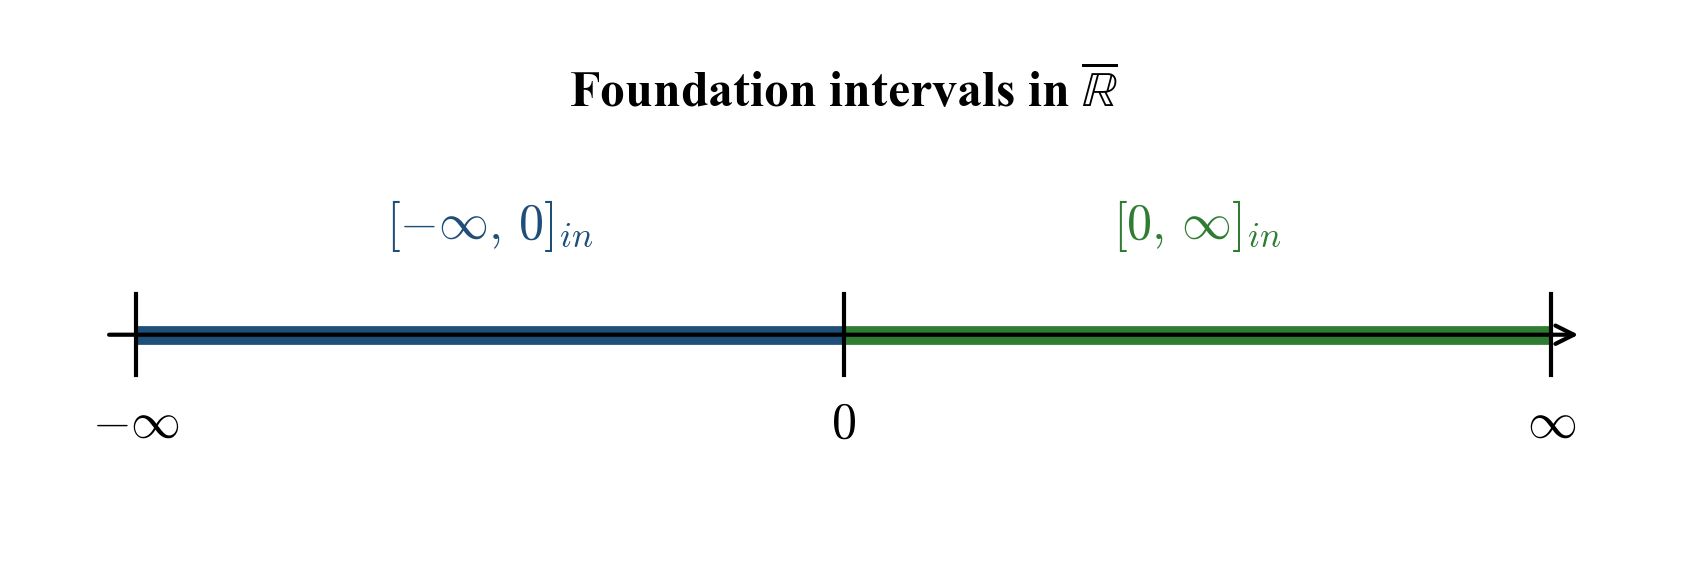
\includegraphics[width=0.85\linewidth]{fig_extended_real_intervals.png}
  \caption{The extended real line $\Rext$ with the two foundation
  intervals $\inI{-\infty, 0}$ (blue) and $\inI{0, \infty}$ (green),
  corresponding to Rules~II and~I, respectively. The intervals are
  not disjoint: they share the point $0$.}
  \label{fig:extended-real-intervals}
\end{figure}

\subsection{Justification for Rules I and II}\label{sec:rule-justification}

The interval representations of Rules I and II are justified by
exhibiting explicit \emph{directional} sequences (with $a_n \ge 0$)
whose products realize a representative spread of limit values within
the intervals. The arguments below show that the assigned intervals
are \emph{attained}; a separate question---whether they are tight,
i.e.\ whether every interior point is attainable as a limit---is
addressed by the parametric witness below.

\paragraph{For $0^{+} \cdot \infty$:}
\begin{itemize}[leftmargin=2em]
  \item Sequence A: $a_n = \tfrac{1}{n^2}$, $b_n = n$.
    Then $a_n b_n = \tfrac{1}{n} \to 0$.
  \item Sequence B: $a_n = \tfrac{1}{n}$, $b_n = n$.
    Then $a_n b_n = 1$ for all $n$.
  \item Sequence C: $a_n = \tfrac{1}{n}$, $b_n = n^2$.
    Then $a_n b_n = n \to \infty$.
\end{itemize}

A parametric witness for any $c \in [0, \infty)$ is $a_n = c/n$,
$b_n = n$, giving $a_n b_n = c$ for all $n$; together with Sequence C,
this shows every value of $\inI{0, \infty}$ is attainable as a limit.

\begin{figure}[H]
  \centering
  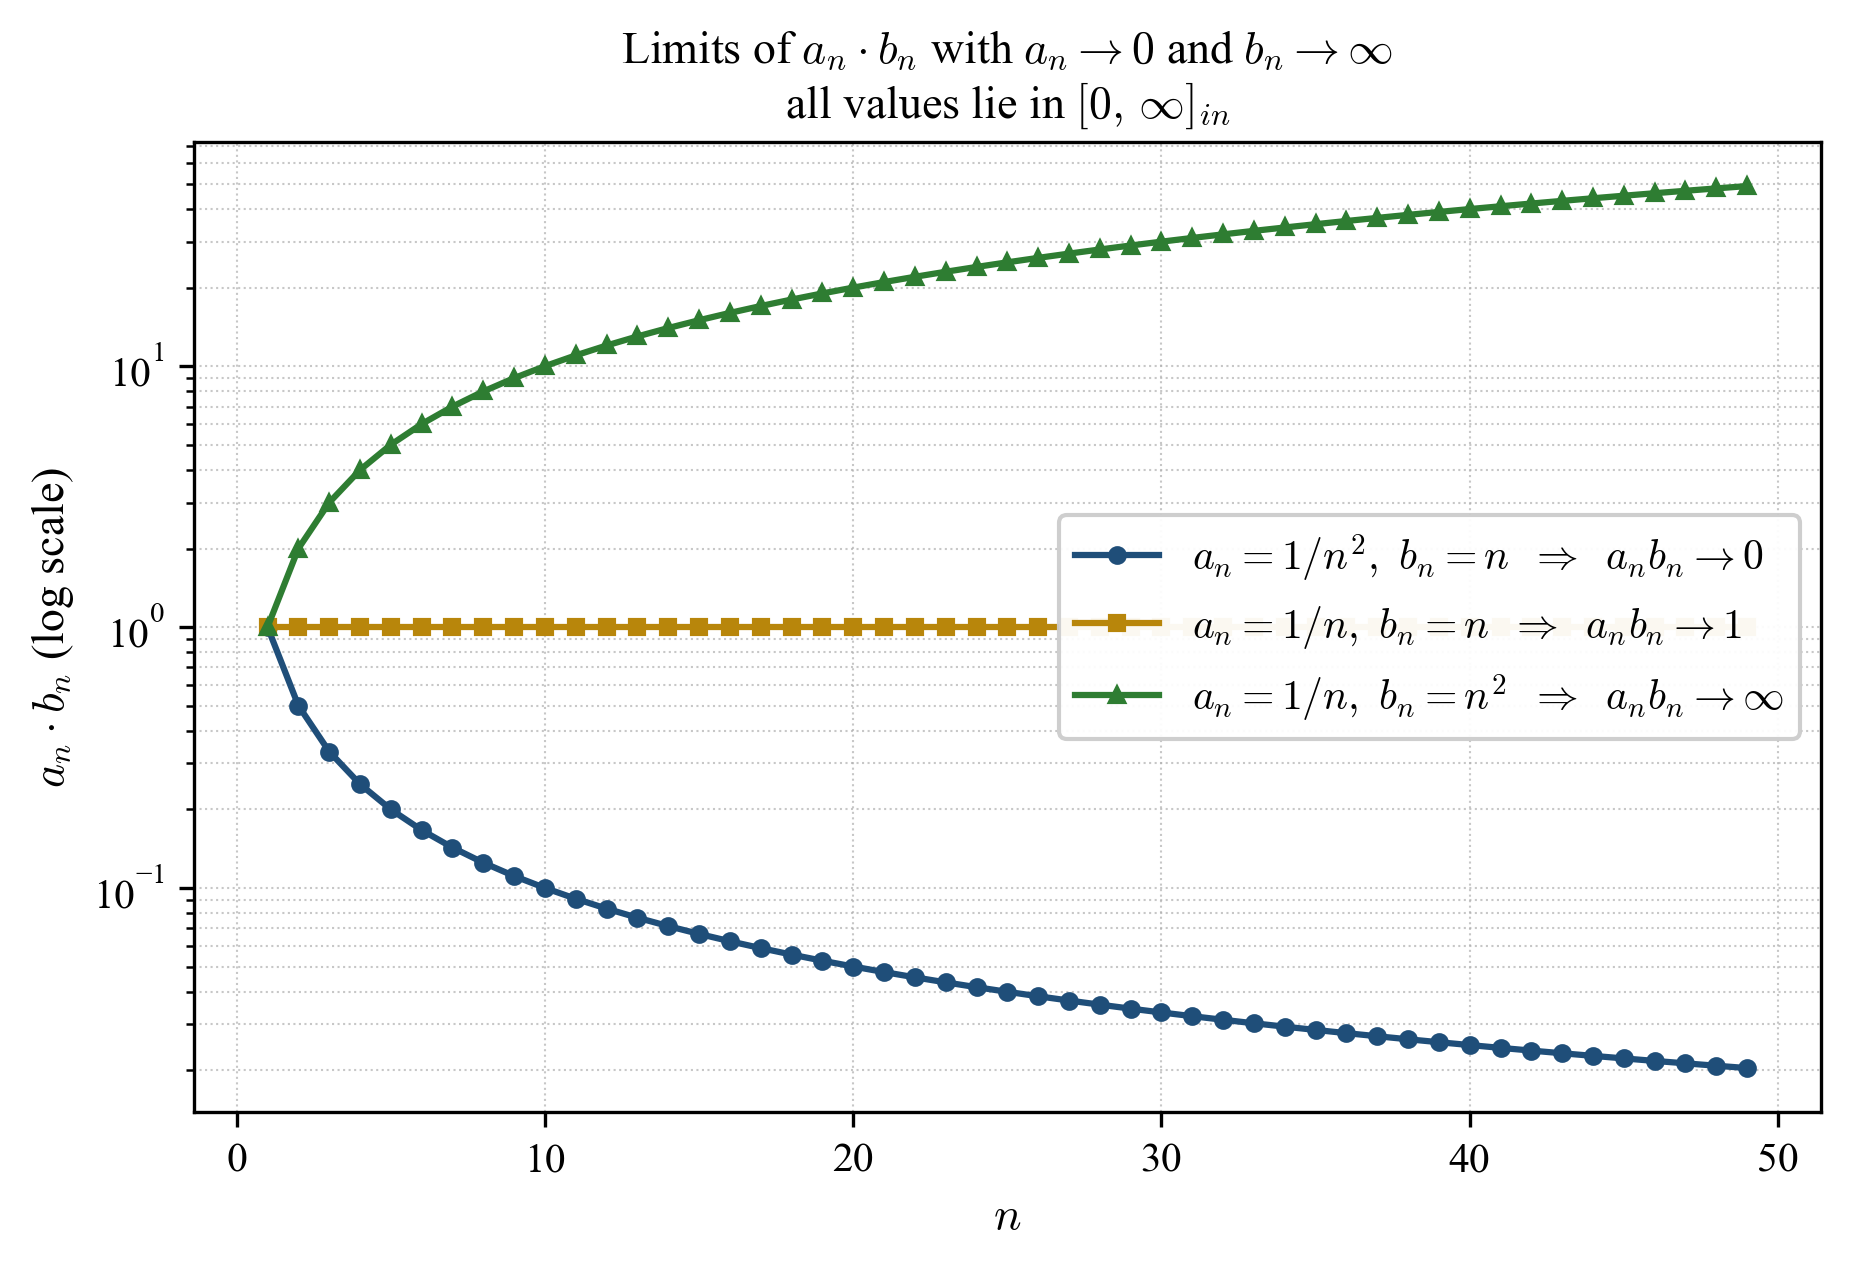
\includegraphics[width=0.75\linewidth]{fig_indeterminate_limits.png}
  \caption{Three sequences $a_n b_n$ with $a_n \to 0^{+}$ and
  $b_n \to \infty$, converging to $0$, $1$, and $\infty$, respectively
  (log-scaled vertical axis). All limit values lie within
  $\inI{0, \infty}$, consistent with Rule~I.}
  \label{fig:indeterminate-limits}
\end{figure}

\paragraph{For $0^{+} \cdot (-\infty)$:}
\begin{itemize}[leftmargin=2em]
  \item Sequence A: $a_n = \tfrac{1}{n}$, $b_n = -n$.
    Then $a_n b_n = -1$ for all $n$.
  \item Sequence B: $a_n = \tfrac{1}{n}$, $b_n = -n^2$.
    Then $a_n b_n = -n \to -\infty$.
\end{itemize}

For any $c \in (-\infty, 0]$, the parametric sequences $a_n = -c/n$,
$b_n = -n$ (with $a_n \ge 0$ since $c \le 0$) give $a_n b_n = c$ for
all $n$, completing the witness for $\inI{-\infty, 0}$.

\begin{proposition}[Tightness of the foundation intervals]\label{prop:foundation-tight}
Let
\[
L^{+} \;:=\; \{\, \lim_{n} a_n b_n \;:\; a_n \ge 0,\ a_n \to 0,\
  b_n \to +\infty,\ \text{and the limit exists in $\Rext$} \,\},
\]
and let $L^{-}$ be defined analogously with $b_n \to -\infty$ in place
of $b_n \to +\infty$. Then
\[
\mathrm{Hull}(L^{+}) \;=\; \inI{0, \infty}, \qquad
\mathrm{Hull}(L^{-}) \;=\; \inI{-\infty, 0}.
\]
\end{proposition}

\begin{proof}
\emph{Containment $L^{+} \subseteq [0, \infty]$.} For each $n$ with
$n$ large enough that $b_n > 0$, the product $a_n b_n \ge 0$ since
$a_n \ge 0$. Hence every existing limit $\lim_n a_n b_n$ lies in
$[0, +\infty]$.

\emph{Attainment of $[0, +\infty]$.} The witnesses in
Section~\ref{sec:rule-justification} show $0, +\infty \in L^{+}$, and
the parametric witness $a_n = c/n,\ b_n = n$ shows $c \in L^{+}$ for
every $c \in [0, +\infty)$. Hence $L^{+} \supseteq [0, +\infty]$, and
combined with the containment, $L^{+} = [0, +\infty]$. Therefore
$\mathrm{Hull}(L^{+}) = [\inf L^{+}, \sup L^{+}] = [0, +\infty]$.

The argument for $L^{-}$ is symmetric: $a_n b_n \le 0$ for large $n$
since $a_n \ge 0$ and $b_n < 0$; the witnesses of
Section~\ref{sec:rule-justification} attain every value of
$[-\infty, 0]$. Hence $\mathrm{Hull}(L^{-}) = [-\infty, 0]$.
\end{proof}

Proposition~\ref{prop:foundation-tight} shows that under the
directional convention of Section~\ref{sec:foundation-rules}, the
foundation intervals are not arbitrary symbolic choices: they are the
unique closed-interval hulls of the directional limit sets, and no
strictly smaller closed interval would contain all admissible limit
values.

%====================================================================
\section{Operations on Interval Numbers}\label{sec:operations}

All operations follow standard interval arithmetic~\cite{Moore1966},
with explicit treatment of indeterminate forms.

\subsection{Multiplication}\label{sec:multiplication}

\begin{definition}[Interval Multiplication]\label{def:multiplication}
For interval numbers $I = \inI{x_0, x_1}$ and $J = \inI{y_0, y_1}$,
define the \emph{candidate set}
\[
\Cand(I, J) \;:=\; \bigcup_{i,j \in \{0,1\}} \V(x_i,\, y_j)
\;\subseteq\; \Rext,
\]
where the \emph{value map} $\V : \Rext \times \Rext \to
\mathcal{P}_{\mathrm{fin}}(\Rext) \setminus \{\emptyset\}$ is defined
on each ordered pair of factors by
\[
\V(a, b) \;:=\;
\begin{cases}
\{a \cdot b\}, & a \cdot b \text{ is defined in $\Rext$}, \\
\{0, \infty\},  & \{a, b\} = \{0, +\infty\}\ \text{(Rule~I)}, \\
\{-\infty, 0\}, & \{a, b\} = \{0, -\infty\}\ \text{(Rule~II)}.
\end{cases}
\]
The product is then
\[
I \cdot J \;:=\; \mathrm{Hull}\bigl(\Cand(I, J)\bigr).
\]
\end{definition}

Multiplication of finite reals with $\pm\infty$ commutes in $\Rext$,
so the value map $\V$ is symmetric in its two arguments. The endpoint
sets $\{0, \infty\}$ and $\{-\infty, 0\}$ returned by $\V$ on
indeterminate factor pairs are exactly the endpoints of the foundation
intervals $\Omega = \inI{0, \infty}$ and $-\Omega = \inI{-\infty, 0}$
of Section~\ref{sec:foundation-rules}; the hull recovers those
intervals.

In particular, if no endpoint product $x_i \cdot y_j$ is an
indeterminate form, the definition reduces to the classical
interval-arithmetic formula
\[
I \cdot J = \inI{\min(x_0 y_0, x_0 y_1, x_1 y_0, x_1 y_1),\
\max(x_0 y_0, x_0 y_1, x_1 y_0, x_1 y_1)}.
\]

\paragraph{Scalar multiplication.} For finite $r \in \mathbb{R}$
identified with the point interval $\inI{r, r}$,
Definition~\ref{def:multiplication} specializes to:
\[
r \cdot \inI{x_0, x_1} =
\begin{cases}
\inI{r x_0,\ r x_1}, & r > 0, \\
\inI{r x_1,\ r x_0}, & r < 0, \\
\inI{0, 0}, & r = 0,\ x_0 > -\infty,\ x_1 < +\infty, \\
\inI{-\infty, 0}, & r = 0,\ x_0 = -\infty,\ x_1 < +\infty, \\
\inI{0, \infty}, & r = 0,\ x_0 > -\infty,\ x_1 = +\infty, \\
\inI{-\infty, \infty}, & r = 0,\ x_0 = -\infty,\ x_1 = +\infty.
\end{cases}
\]
The four $r = 0$ subcases follow from $\V$ applied to the factor pairs
$(0, x_0)$ and $(0, x_1)$. For \emph{infinite} scalars
$r \in \{-\infty, +\infty\}$ (which may produce indeterminate factor
pairs $(r, 0)$ when $0 \in [x_0, x_1]$), no closed-form
simplification is asserted; the result is obtained directly from the
candidate-set rule of Definition~\ref{def:multiplication}, e.g.
\[
+\infty \cdot \inI{0, 1}
\;=\; \mathrm{Hull}\bigl(\V(+\infty, 0) \cup \V(+\infty, 1)\bigr)
\;=\; \mathrm{Hull}(\{0, +\infty\})
\;=\; \inI{0, +\infty}.
\]

\paragraph{Geometric interpretation.} The four endpoint products
correspond to the corners of the rectangle $[x_0, x_1] \times [y_0, y_1]$
in the $xy$-plane:

\begin{figure}[H]
  \centering
  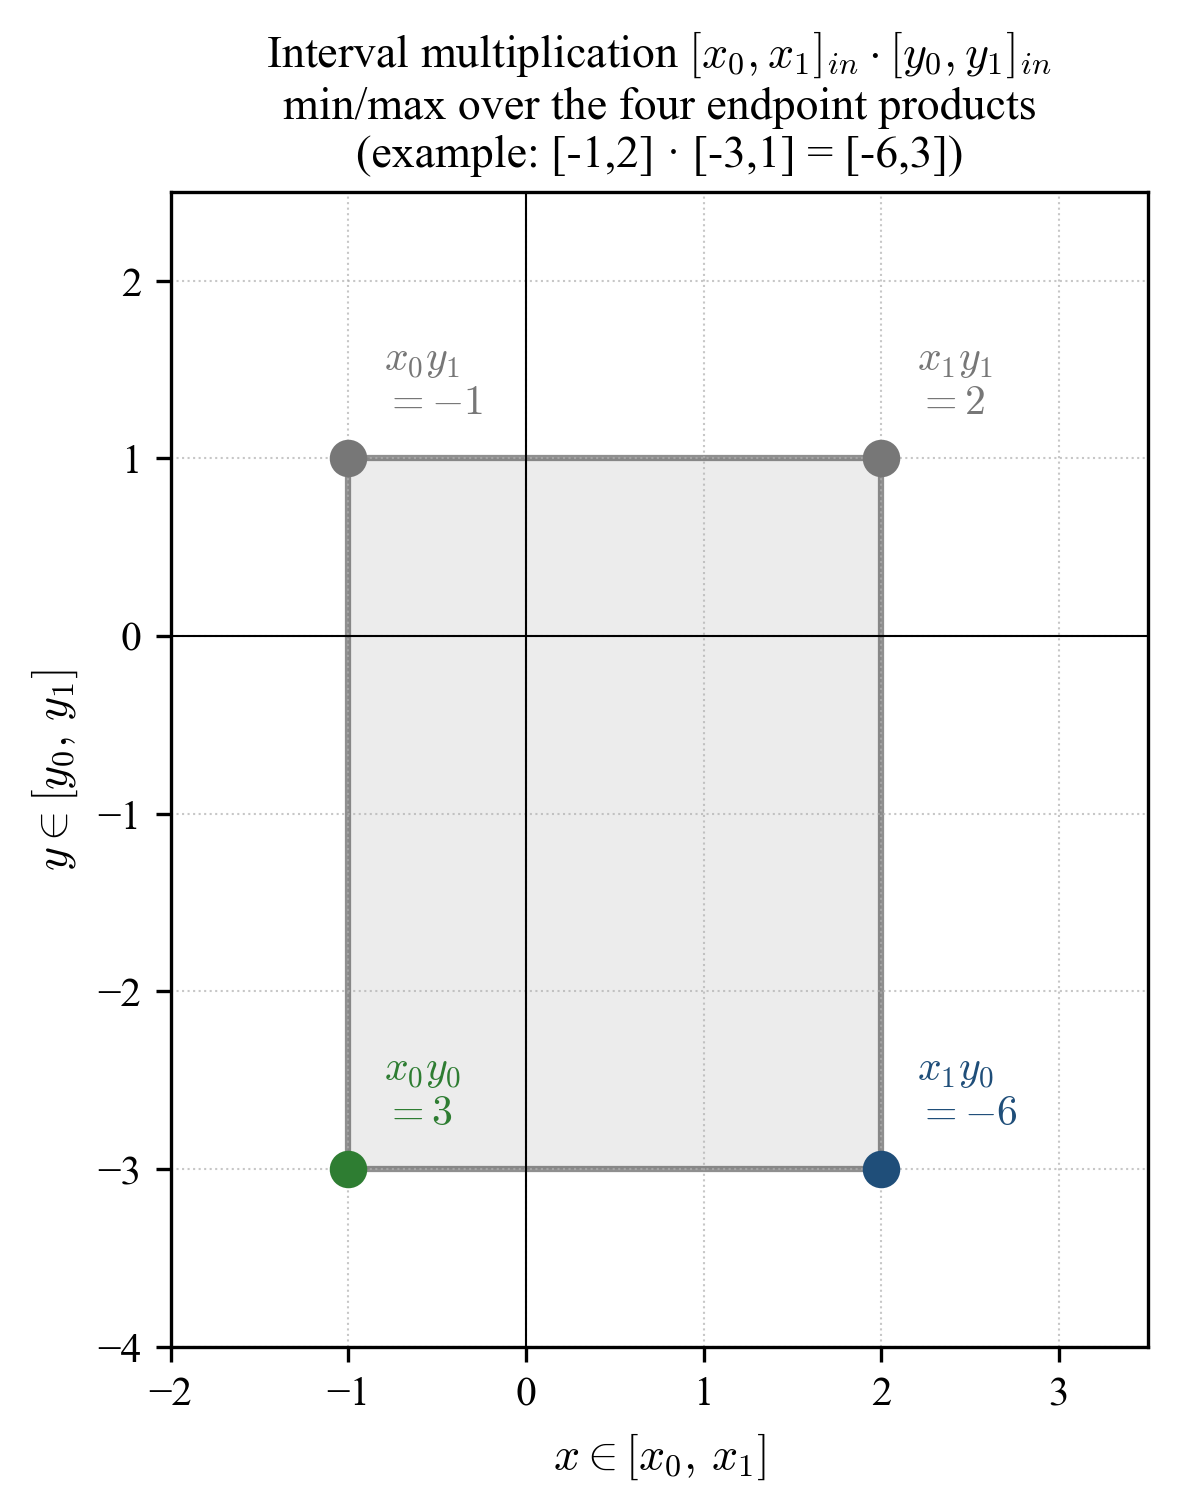
\includegraphics[width=0.7\linewidth]{fig_interval_multiplication.png}
  \caption{Geometric view of interval multiplication. The product
  $\inI{x_0, x_1} \cdot \inI{y_0, y_1}$ is the closed interval bounded
  by the minimum and maximum of the four corner products. Example:
  $\inI{-1, 2} \cdot \inI{-3, 1} = \inI{-6, 3}$.}
  \label{fig:interval-multiplication}
\end{figure}

\paragraph{Examples.}
\begin{itemize}[leftmargin=2em]
  \item $(-1) \cdot \inI{0, \infty} = \inI{-\infty, 0}$
    (validates the consistency between Rule~I and Rule~II).
  \item $2 \cdot \inI{1, 3} = \inI{2, 6}$.
\end{itemize}

\subsection{Addition}\label{sec:addition}

\begin{definition}[Interval Addition]\label{def:addition}
For interval numbers $I = \inI{x_0, x_1}$ and $J = \inI{y_0, y_1}$,
define the candidate set
\[
\Cand_{+}(I, J) \;:=\; \V_{+}(x_0,\, y_0) \cup \V_{+}(x_1,\, y_1)
\;\subseteq\; \Rext,
\]
where the additive value map $\V_{+} : \Rext \times \Rext \to
\mathcal{P}_{\mathrm{fin}}(\Rext) \setminus \{\emptyset\}$ is
\[
\V_{+}(a, b) \;:=\;
\begin{cases}
\{a + b\}, & a + b \text{ is defined in $\Rext$}, \\
\{-\infty, \infty\}, & \{a, b\} = \{+\infty, -\infty\}.
\end{cases}
\]
Then
\[
I + J \;:=\; \mathrm{Hull}\bigl(\Cand_{+}(I, J)\bigr).
\]
\end{definition}

When neither endpoint sum is indeterminate this reduces to
$\inI{x_0 + y_0,\ x_1 + y_1}$.

\paragraph{Example.} $\inI{0, \infty} + 5 = \inI{5, \infty}$.
$\inI{0, \infty} + \inI{-\infty, 0} = \inI{-\infty, \infty}$.

\subsection{Subtraction}\label{sec:subtraction}

\begin{definition}[Interval Subtraction]\label{def:subtraction}
Let the subtractive value map $\V_{-} : \Rext \times \Rext \to
\mathcal{P}_{\mathrm{fin}}(\Rext) \setminus \{\emptyset\}$ be
\[
\V_{-}(a, b) \;:=\;
\begin{cases}
\{a - b\}, & a - b \text{ is defined in $\Rext$}, \\
\{-\infty, \infty\}, & a = b \in \{+\infty, -\infty\}.
\end{cases}
\]
Define
\[
\Cand_{-}(I, J) \;:=\; \V_{-}(x_0,\, y_1) \cup \V_{-}(x_1,\, y_0),
\qquad
I - J \;:=\; \mathrm{Hull}\bigl(\Cand_{-}(I, J)\bigr).
\]
\end{definition}

When no indeterminate form arises this reduces to
$\inI{x_0 - y_1,\ x_1 - y_0}$.

\paragraph{Example.} $\inI{1, 5} - \inI{2, 3} = \inI{-2, 3}$.

\subsection{Reciprocal}\label{sec:reciprocal}

\begin{definition}[Reciprocal]\label{def:reciprocal}
Reciprocation is defined on all of $\Iset$ by the following case
analysis on the divisor $J = \inI{y_0, y_1}$:
\[
\frac{1}{J} :=
\begin{cases}
\inI{-\infty, \infty}, & y_0 = y_1 = 0, \\
\inI{\tfrac{1}{y_1},\ \tfrac{1}{y_0}}, & y_0 > 0 \text{ or } y_1 < 0, \\
\inI{\tfrac{1}{y_1},\ +\infty}, & y_0 = 0,\; y_1 > 0, \\
\inI{-\infty,\ \tfrac{1}{y_0}}, & y_0 < 0,\; y_1 = 0, \\
\inI{-\infty, \infty}, & y_0 < 0 < y_1.
\end{cases}
\]
\end{definition}

The conventions $1/(0^{+}) = +\infty$ and $1/(0^{-}) = -\infty$
follow from one-sided real limits; the assignment for
$J = \inI{0, 0}$ is by convention, since neither sign of approach is
privileged for a point interval at zero.

When $y_0 < 0 < y_1$, the exact reciprocal is the union of two
unbounded branches
$\inI{-\infty, 1/y_0} \cup \inI{1/y_1, +\infty}$, which is not a single
interval. The framework returns its convex hull
$\inI{-\infty, \infty}$, retaining closure within $\Iset$ at the cost
of tightness.

\begin{figure}[H]
  \centering
  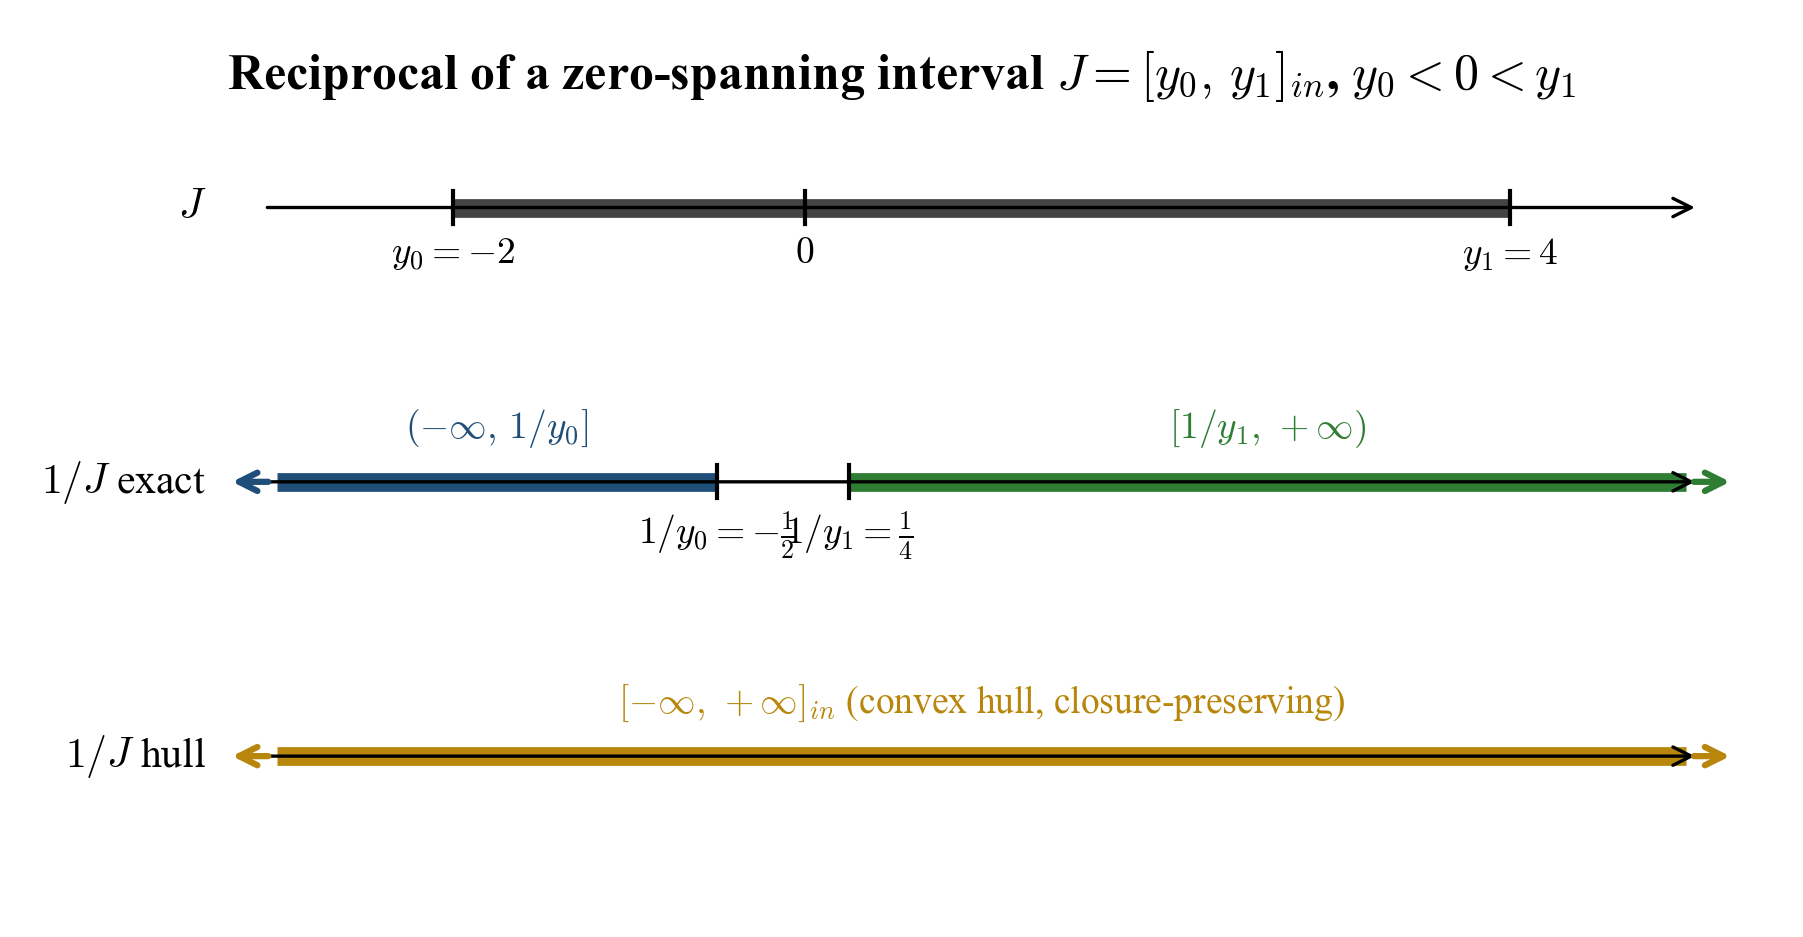
\includegraphics[width=0.8\linewidth]{fig_reciprocal_zero_spanning.png}
  \caption{Reciprocal of a zero-spanning interval
  $J = \inI{y_0, y_1}$ with $y_0 < 0 < y_1$ (example
  $J = \inI{-2, 4}$). The exact reciprocal consists of two unbounded
  branches $(-\infty, 1/y_0]$ and $[1/y_1, +\infty)$ separated by a
  gap; the framework replaces this non-convex set with its convex
  hull $\inI{-\infty, +\infty}$ to preserve closure within $\Iset$.}
  \label{fig:reciprocal}
\end{figure}

\subsection{Division}\label{sec:division}

\begin{definition}[Interval Division]\label{def:division}
Division is defined on all of $\Iset \times \Iset$ by
\[
I \div J := I \cdot \frac{1}{J},
\]
evaluated using Definition~\ref{def:multiplication} and
Definition~\ref{def:reciprocal}. The case analysis of the reciprocal
makes division a total operation on $\Iset$.
\end{definition}

\paragraph{Indeterminate form $\tfrac{0}{0}$.} With
$I = J = \inI{0, 0}$, Definition~\ref{def:reciprocal} gives
$1/J = \inI{-\infty, \infty}$, and then
$\inI{0, 0} \cdot \inI{-\infty, \infty} = \inI{-\infty, \infty}$ via
Rules I and II in Definition~\ref{def:multiplication}.

This is consistent with the one-sided limit witnesses
\[
\lim_{x \to 0^{+}} \frac{x}{x^{2}} = +\infty, \qquad
\lim_{x \to 0^{-}} \frac{x}{x^{2}} = -\infty,
\]
and the parametric witness $a_n = c/n$, $b_n = 1/n$ giving
$a_n / b_n = c$ for any $c \in \mathbb{R}$.

\paragraph{Indeterminate form $\tfrac{\infty}{\infty}$.} With
$I = J = \inI{\infty, \infty}$, Definition~\ref{def:reciprocal} gives
$1/J = \inI{0, 0}$, and then
$\inI{\infty, \infty} \cdot \inI{0, 0} = \inI{0, \infty}$ via Rule I
in Definition~\ref{def:multiplication}.

\subsection{Absolute Value}\label{sec:absolute-value}

\begin{definition}[Absolute Value]\label{def:abs}
Absolute value is defined by order rather than by endpoint
multiplication, so that no indeterminate product is required:
\[
\lvert \inI{x_0, x_1} \rvert :=
\begin{cases}
\inI{x_0,\ x_1}, & 0 \le x_0, \\
\inI{-x_1,\ -x_0}, & x_1 \le 0, \\
\inI{0,\ \max(-x_0,\ x_1)}, & x_0 < 0 < x_1.
\end{cases}
\]
\end{definition}

Negation of $\pm\infty$ is interpreted in $\Rext$ in the standard way.

\paragraph{Examples.}
$\lvert \inI{-5, 3} \rvert = \inI{0, 5}$.
$\lvert \inI{-\infty, 0} \rvert = \inI{0, \infty}$.
$\lvert \inI{0, \infty} \rvert = \inI{0, \infty}$.

\subsection{Exponentiation}\label{sec:exponentiation}

\begin{definition}[Power]\label{def:power}
Let $I = \inI{x_0, x_1}$ and $E = \inI{y_0, y_1}$. The
\emph{admissible domain} of exponentiation is
\begin{align*}
\mathrm{dom}(\,\cdot^{\,\cdot}) := \{\, (I, E) \in \Iset \times \Iset \;:\;
& (x_0 > 0) \;\text{or}\; (x_0 \ge 0\ \text{and}\ y_0 \ge 0)\\
& \text{or}\; (E = \{n\},\ n \in \mathbb{Z}_{\ge 0})\\
& \text{or}\; (E = \{n\},\ n \in \mathbb{Z}_{<0}\ \text{and}\ 0 \notin I)\,\}.
\end{align*}
On the admissible domain, exponentiation is defined as the closed
interval hull of the image set:
\[
I^{E} \;:=\; \mathrm{Hull}\bigl(\mathcal{S}(I, E)\bigr),
\]
where
\[
\mathcal{S}(I, E) \;:=\; \bigcup_{x \in I,\ y \in E} \Vhat(x,\, y)
\;\subseteq\; \Rext,
\]
and the exponentiation value map $\Vhat$ is the \emph{partial} map
$\Rext \times \Rext \rightharpoonup
\mathcal{P}_{\mathrm{fin}}(\Rext) \setminus \{\emptyset\}$, defined
exactly on the pairs falling into one of the two cases below, that
extends real-valued exponentiation by handling the
indeterminate-form points:
\[
\Vhat(b, e) \;:=\;
\begin{cases}
\{0, \infty\}, & (b, e) \in \{(0,0),\ (1, +\infty),\ (1, -\infty),
\ (+\infty, 0),\ (-\infty, 0)\}, \\
\{b^{e}\}, & b^{e} \text{ is defined in } \Rext.
\end{cases}
\]
On the admissible domain, every pair $(x, y) \in I \times E$ lies in
the domain of $\Vhat$, so $\mathcal{S}(I, E)$ is a nonempty subset of
$\Rext$ and $I^{E} = \mathrm{Hull}(\mathcal{S}(I, E))$ is an interval
number by Proposition~\ref{prop:hull}. Moreover, the hull endpoints
are \emph{attained} in $\mathcal{S}(I, E)$: the real-valued
continuous map $(x, y) \mapsto x^{y}$ is monotone in each argument on
each of the rectangles obtained by splitting $I \times E$ along
$x = 1$ and $y = 0$, so its image is a closed interval, and the
finitely many indeterminate-form contributions of $\Vhat$ only add
isolated endpoint values.
\end{definition}

That is, exponentiation is admitted when (i) the base interval is
strictly positive, or (ii) the base interval is non-negative and the
exponent interval is non-negative (so no $0^{y}$ with $y < 0$
arises), or (iii) the exponent is a single non-negative integer (so
negative bases are handled by integer powers and zero bases give
$0^{n} = 0$ for $n \ge 1$ and $0^{0}$ via $\Vhat$), or (iv) the
exponent is a single negative integer and $0 \notin I$ (so $0^{n}$
with $n < 0$ does not arise).

The admissible domain is chosen precisely so that every pair
$(x, y) \in I \times E$ falls into one of the two cases above; in
particular, points $0^{y}$ with $y < 0$ are excluded by the domain
restriction (i)--(iv). If $(I, E) \notin \mathrm{dom}(\,\cdot^{\,\cdot})$
the operation is mathematically undefined; the reference
implementation tests membership in the admissible domain explicitly
and returns NaN for any pair lying outside it.

\paragraph{Reduction to corner formulas.} On regions where
$x \mapsto x^y$ and $y \mapsto x^y$ are jointly monotonic, the
supremum and infimum of $\mathcal{S}(I, E)$ are attained at corners
$(x_i, y_j)$ and Definition~\ref{def:power} reduces to a four-corner
endpoint formula. This is \emph{not} the case in general; in
particular, for a point positive-integer exponent $E = \{n\}$ with
$n \in \mathbb{Z}_{>0}$ and a base interval crossing zero,
$x \mapsto x^n$ attains its minimum $0$ in the interior:
\[
\inI{x_0, x_1}^{\{n\}} =
\begin{cases}
\inI{x_0^{n},\ x_1^{n}}, & 0 \le x_0\ \text{or}\ n\ \text{odd}, \\
\inI{x_1^{n},\ x_0^{n}}, & x_1 \le 0\ \text{and}\ n\ \text{even}, \\
\inI{0,\ \max(x_0^{n},\ x_1^{n})}, & x_0 < 0 < x_1\ \text{and}\ n\ \text{even},
\end{cases}
\qquad (n \in \mathbb{Z}_{>0}).
\]

The case $n = 0$ is \emph{not} covered by the formula above: if $I$
contains an indeterminate base for the exponent $0$---that is, if
$0 \in I$ (giving the pair $(0, 0)$) or if $\pm\infty \in I$ (giving
the pair $(\pm\infty, 0)$)---then $\Vhat$ contributes
$\{0, \infty\}$ at that point and $I^{\{0\}} = \inI{0, \infty}$;
otherwise every point of $I$ is finite and nonzero, $b^{0} = 1$
pointwise, and $I^{\{0\}} = \inI{1, 1}$. The case
$n \in \mathbb{Z}_{<0}$ is admissible only when $0 \notin I$ (case
(iv) above); on that region $x \mapsto x^n$ is monotone and the
result is
\[
\inI{x_0, x_1}^{\{n\}}
\;=\; \inI{\min(x_0^n, x_1^n),\ \max(x_0^n, x_1^n)},
\qquad (n \in \mathbb{Z}_{<0},\ 0 \notin I).
\]

For strictly positive finite base intervals $I \subseteq (0, +\infty)$,
write $x^{y} = \exp(y \log x)$. The image $y \log x$ over
$\log I \times E$ is determined by the standard interval-product hull
on these finite quantities, and applying the increasing map $\exp$
yields the corresponding hull for $x^{y}$. The only indeterminate
closure point that can arise in this case is $1^{\pm\infty}$ (when
$1 \in I$ and $\pm\infty \in E$), which is supplemented via $\Vhat$;
the extended-base indeterminate pair $(\pm\infty, 0)$ does not
arise here and is handled by the general image-set definition above.

\paragraph{Indeterminate forms.}
\[
0^{0} = 1^{\infty} = \infty^{0} = \inI{0, \infty}.
\]
Each of these arises as $\Vhat$ applied to the corresponding
indeterminate-form point. The signed variants admitted by
Definition~\ref{def:power}---namely $1^{-\infty}$ and
$(-\infty)^{0}$---are also indeterminate and receive the same hull
$\inI{0, \infty}$ by formal assignment via $\Vhat$. For
$1^{-\infty}$, the parametric sequence
$a_n = 1 + (\ln c)/n,\ b_n = -n$ gives $a_n^{b_n} \to c^{-1}$,
attaining every $c^{-1} \in (0, \infty)$ as $c$ varies, so
$\inI{0, \infty}$ is a genuine limit hull. For $(-\infty)^{0}$, no
analogous real-valued limit-witness argument is claimed: non-integer
real exponents of negative bases are not real-valued, so
$(-\infty)^{0} = \inI{0, \infty}$ is a \emph{formal convention} of
the value map $\Vhat$ adopted for symmetry with $(+\infty)^{0}$ and
to keep the admissible domain closed under sign reflection of the
base.

\paragraph{Justification of $0^{0} = \inI{0, \infty}$:}
\begin{itemize}[leftmargin=2em]
  \item Sequence A: $a_n = 1/n$, $b_n = 1/\sqrt{\ln n}$, then
    $a_n^{b_n} \to 0$.
  \item Sequence B: $a_n = 1/n$, $b_n = 1/\ln n$, then
    $a_n^{b_n} \to e^{-1}$.
  \item Sequence C: $a_n = 1/n$, $b_n = -1/\sqrt{\ln n}$, then
    $a_n^{b_n} \to \infty$.
  \item For any $c > 0$, the parametric witness $a_n = 1/n$,
    $b_n = -\ln c / \ln n$ gives $a_n^{b_n} = c$ for all $n \ge 2$,
    so every value of $(0, \infty)$ is attained.
\end{itemize}

%====================================================================
\section{Algebraic Structure}\label{sec:algebraic-structure}

This section examines the algebraic structure induced by
interval-number operations, with emphasis on which classical axioms
hold and which fail.

\subsection{Closure under Multiplication}\label{sec:closure}

\begin{theorem}[Closure]\label{thm:closure}
The set of interval numbers $\Iset$, equipped with the multiplication
operation of Definition~\ref{def:multiplication}, forms a
\emph{unital magma}~\cite{MacLaneBirkhoff1999}: it is closed under
multiplication, with two-sided identity $\inI{1, 1}$.
\end{theorem}

\begin{proof}[Proof of closure]
A magma is a set with a single binary operation that is
closed~\cite{Bourbaki1989,MacLaneBirkhoff1999}. Let
$I = \inI{x_0, x_1}$ and $J = \inI{y_0, y_1}$ be interval numbers,
with $x_0, x_1, y_0, y_1 \in \Rext$. For each of the four ordered
pairs $(x_i, y_j)$ with $i, j \in \{0, 1\}$, the product
$x_i \cdot y_j$ is either:
\begin{enumerate}[label=(\alph*),leftmargin=2em]
  \item a defined element of $\Rext$, in which case
    $\V(x_i, y_j) = \{x_i \cdot y_j\}$ is a singleton; or
  \item an indeterminate pair $\{x_i, y_j\} = \{0, \pm\infty\}$, in
    which case Rules~I and~II assign
    $\V(x_i, y_j) \in \{\{0, \infty\},\ \{-\infty, 0\}\}$, a finite
    two-element subset of $\Rext$.
\end{enumerate}
In either case $\V(x_i, y_j)$ is a nonempty finite subset of $\Rext$.
Hence
$\Cand(I, J) = \bigcup_{i,j} \V(x_i, y_j)$ is a nonempty finite
subset of $\Rext$, and by Proposition~\ref{prop:hull},
$I \cdot J = \mathrm{Hull}(\Cand(I, J)) \in \Iset$. This establishes
closure.
\end{proof}

\begin{proof}[Proof of identity]
For $I = \inI{x_0, x_1}$ with $x_0, x_1 \in \Rext$, the factor pairs
in $\inI{1, 1} \cdot I$ are $(1, x_0)$ and $(1, x_1)$ (each appearing
twice). Since one factor is the finite nonzero scalar $1$, no
indeterminate pair $\{0, \pm\infty\}$ arises, and each product is
defined in $\Rext$ with $1 \cdot x_i = x_i$. Hence
$\Cand(\inI{1,1}, I) = \{x_0, x_1\}$ and
\[
\inI{1, 1} \cdot I \;=\; \mathrm{Hull}(\{x_0, x_1\})
\;=\; \inI{x_0, x_1} \;=\; I.
\]
The argument for $I \cdot \inI{1, 1}$ is symmetric, since $\V$ is
symmetric in its arguments. Uniqueness: if $\inI{e_0, e_1}$ is also a
two-sided identity, then
$\inI{e_0, e_1} = \inI{e_0, e_1} \cdot \inI{1, 1} = \inI{1, 1}$, where
the first equality uses that $\inI{1, 1}$ is a right identity and the
second that $\inI{e_0, e_1}$ is a left identity. Hence $\inI{1, 1}$
is the unique two-sided identity.
\end{proof}

\begin{proposition}[Embedding $\Rext \hookrightarrow \Iset$]\label{prop:embedding}
The map $\iota : \Rext \to \Iset,\ r \mapsto \inI{r, r}$ is injective
and satisfies the following compatibility with $\Rext$ arithmetic on
its image. Let $\circ$ denote any of $+,\,-,\,\cdot$ in $\Rext$ and
its lift to $\Iset$ from Section~\ref{sec:operations}. If
$r \circ s$ is defined in $\Rext$, then
$\iota(r) \circ \iota(s) = \iota(r \circ s)$. If $r \circ s$ is
indeterminate, then $\iota(r) \circ \iota(s)$ is the corresponding
foundation interval ($\Omega$, $-\Omega$, or
$\widetilde{\Omega}$).
\end{proposition}

\begin{proof}
Injectivity is immediate from
Definition~\ref{def:point-interval}. For multiplication: if
$r \cdot s$ is defined in $\Rext$, the four factor pairs of
$\iota(r) \cdot \iota(s)$ collapse to a single pair $(r, s)$ with
$\V(r, s) = \{r \cdot s\}$, so $\iota(r) \cdot \iota(s) =
\mathrm{Hull}(\{r \cdot s\}) = \inI{r \cdot s, r \cdot s}
= \iota(r \cdot s)$. If $\{r, s\} = \{0, +\infty\}$ (resp.\
$\{0, -\infty\}$), then $\V(r, s) = \{0, \infty\}$ (resp.\
$\{-\infty, 0\}$), and the hull yields $\Omega$ (resp.\ $-\Omega$).
The arguments for $\pm$ are analogous, with $\V_{+}$ (resp.\
$\V_{-}$) on $\{+\infty, -\infty\}$ producing the full-range
foundation interval $\widetilde{\Omega}$.
\end{proof}

\begin{proposition}[Inclusion monotonicity]\label{prop:monotone}
For each of the binary operations $\circ \in \{+,\, -,\, \cdot\}$
defined in Section~\ref{sec:operations}, and for all
$I, I', J, J' \in \Iset$,
\[
I \subseteq I' \ \text{and}\ J \subseteq J'
\quad\Longrightarrow\quad I \circ J \subseteq I' \circ J'.
\]
The same holds for the unary operation $|\cdot|$
(Definition~\ref{def:abs}) and for exponentiation $I^E$ on pairs
$(I, E), (I', E')$ that both lie in the admissible domain of
Definition~\ref{def:power}. The reciprocal $1/\,\cdot\,$ and division
$\div$ are \emph{not} inclusion-monotone in general; the single
obstruction is the degenerate divisor $\inI{0,0}$, and is described in
Remark~\ref{rem:recip-nonmono} below.
\end{proposition}

\begin{proof}
For each operation $\circ \in \{+, -, \cdot\}$, the result equals the
hull of the \emph{full} image set
$\mathcal{S}_{\circ}(I, J) := \bigcup_{x \in I,\, y \in J}
\V_{\circ}(x, y)$, where $\V_{\circ}$ is the corresponding value map
(Definitions~\ref{def:multiplication}--\ref{def:subtraction}); the
endpoint-only candidate set has the same hull because each value map is
monotone in each argument on the sign-constant subrectangles of
$I \times J$, so its extreme values are attained at endpoints, while
the indeterminate corners contribute exactly the endpoints of the
foundation intervals. If $I \subseteq I'$ and $J \subseteq J'$ then
$\mathcal{S}_{\circ}(I, J) \subseteq \mathcal{S}_{\circ}(I', J')$, and
$\mathrm{Hull}(S) \subseteq \mathrm{Hull}(S')$ whenever
$S \subseteq S'$, so $I \circ J \subseteq I' \circ J'$. The same image-set
argument applies to $|\cdot|$ (whose value at each point is
$\lvert x \rvert$, monotone under inclusion of the operand) and to
exponentiation, whose image set $\mathcal{S}(I, E)$ is by construction
monotone in $(I, E)$ under set inclusion on the admissible domain.
\end{proof}

\begin{remark}[Failure of monotonicity for the reciprocal]\label{rem:recip-nonmono}
Unlike the operations above, the reciprocal of
Definition~\ref{def:reciprocal} is not defined as the hull of a
pointwise image set: the case $J = \inI{0,0}$ is the
\emph{convention} $1/\inI{0,0} := \inI{-\infty, \infty}$
(Section~\ref{sec:limitations}, Limitation~3), which assigns the
\emph{widest} interval to the \emph{narrowest} divisor. This breaks
inclusion monotonicity at exactly that point. For example,
\[
\inI{0,0} \subseteq \inI{0,2},
\quad\text{yet}\quad
\tfrac{1}{\inI{0,0}} = \inI{-\infty, \infty}
\;\not\subseteq\;
\inI{\tfrac12, +\infty} = \tfrac{1}{\inI{0,2}},
\]
and likewise $\inI{0,0} \subseteq \inI{-2,0}$ with
$1/\inI{-2,0} = \inI{-\infty, -\tfrac12}$. Since division is defined
through the reciprocal (Definition~\ref{def:division}), $\div$
inherits the same failure. On all other case boundaries of
Definition~\ref{def:reciprocal} the operation \emph{is} monotone: every
case other than $\inI{0,0}$ returns the hull of the pointwise reciprocal
image, and an exhaustive check over divisor pairs on the endpoint set
$\{-\infty, -2, -1, 0, 1, 2, +\infty\}$ exhibits failures only for the
smaller divisor $\inI{0,0}$. The obstruction is therefore confined to
the single degenerate divisor $\inI{0,0}$.
\end{remark}

\subsection{Failure of Associativity}\label{sec:non-associativity}

\begin{proposition}[Non-associativity]\label{prop:non-assoc}
Multiplication on $\Iset$ is not associative.
\end{proposition}

\begin{proof}[Counterexample]
Let $a = -1$, $b = 0$, $c = -\infty$ (each viewed as a point
interval). Then:
\[
b \cdot c \;=\; 0 \cdot (-\infty) \;=\; \inI{-\infty, 0}
\quad \text{(Rule II)},
\]
\[
a \cdot (b \cdot c) \;=\; -1 \cdot \inI{-\infty, 0}
\;=\; \inI{0, \infty},
\]
while
\[
a \cdot b \;=\; -1 \cdot 0 \;=\; 0,
\]
\[
(a \cdot b) \cdot c \;=\; 0 \cdot (-\infty)
\;=\; \inI{-\infty, 0} \quad \text{(Rule II)}.
\]
Hence
$a \cdot (b \cdot c) = \inI{0, \infty} \ne \inI{-\infty, 0}
= (a \cdot b) \cdot c$.
\end{proof}

\begin{figure}[H]
  \centering
  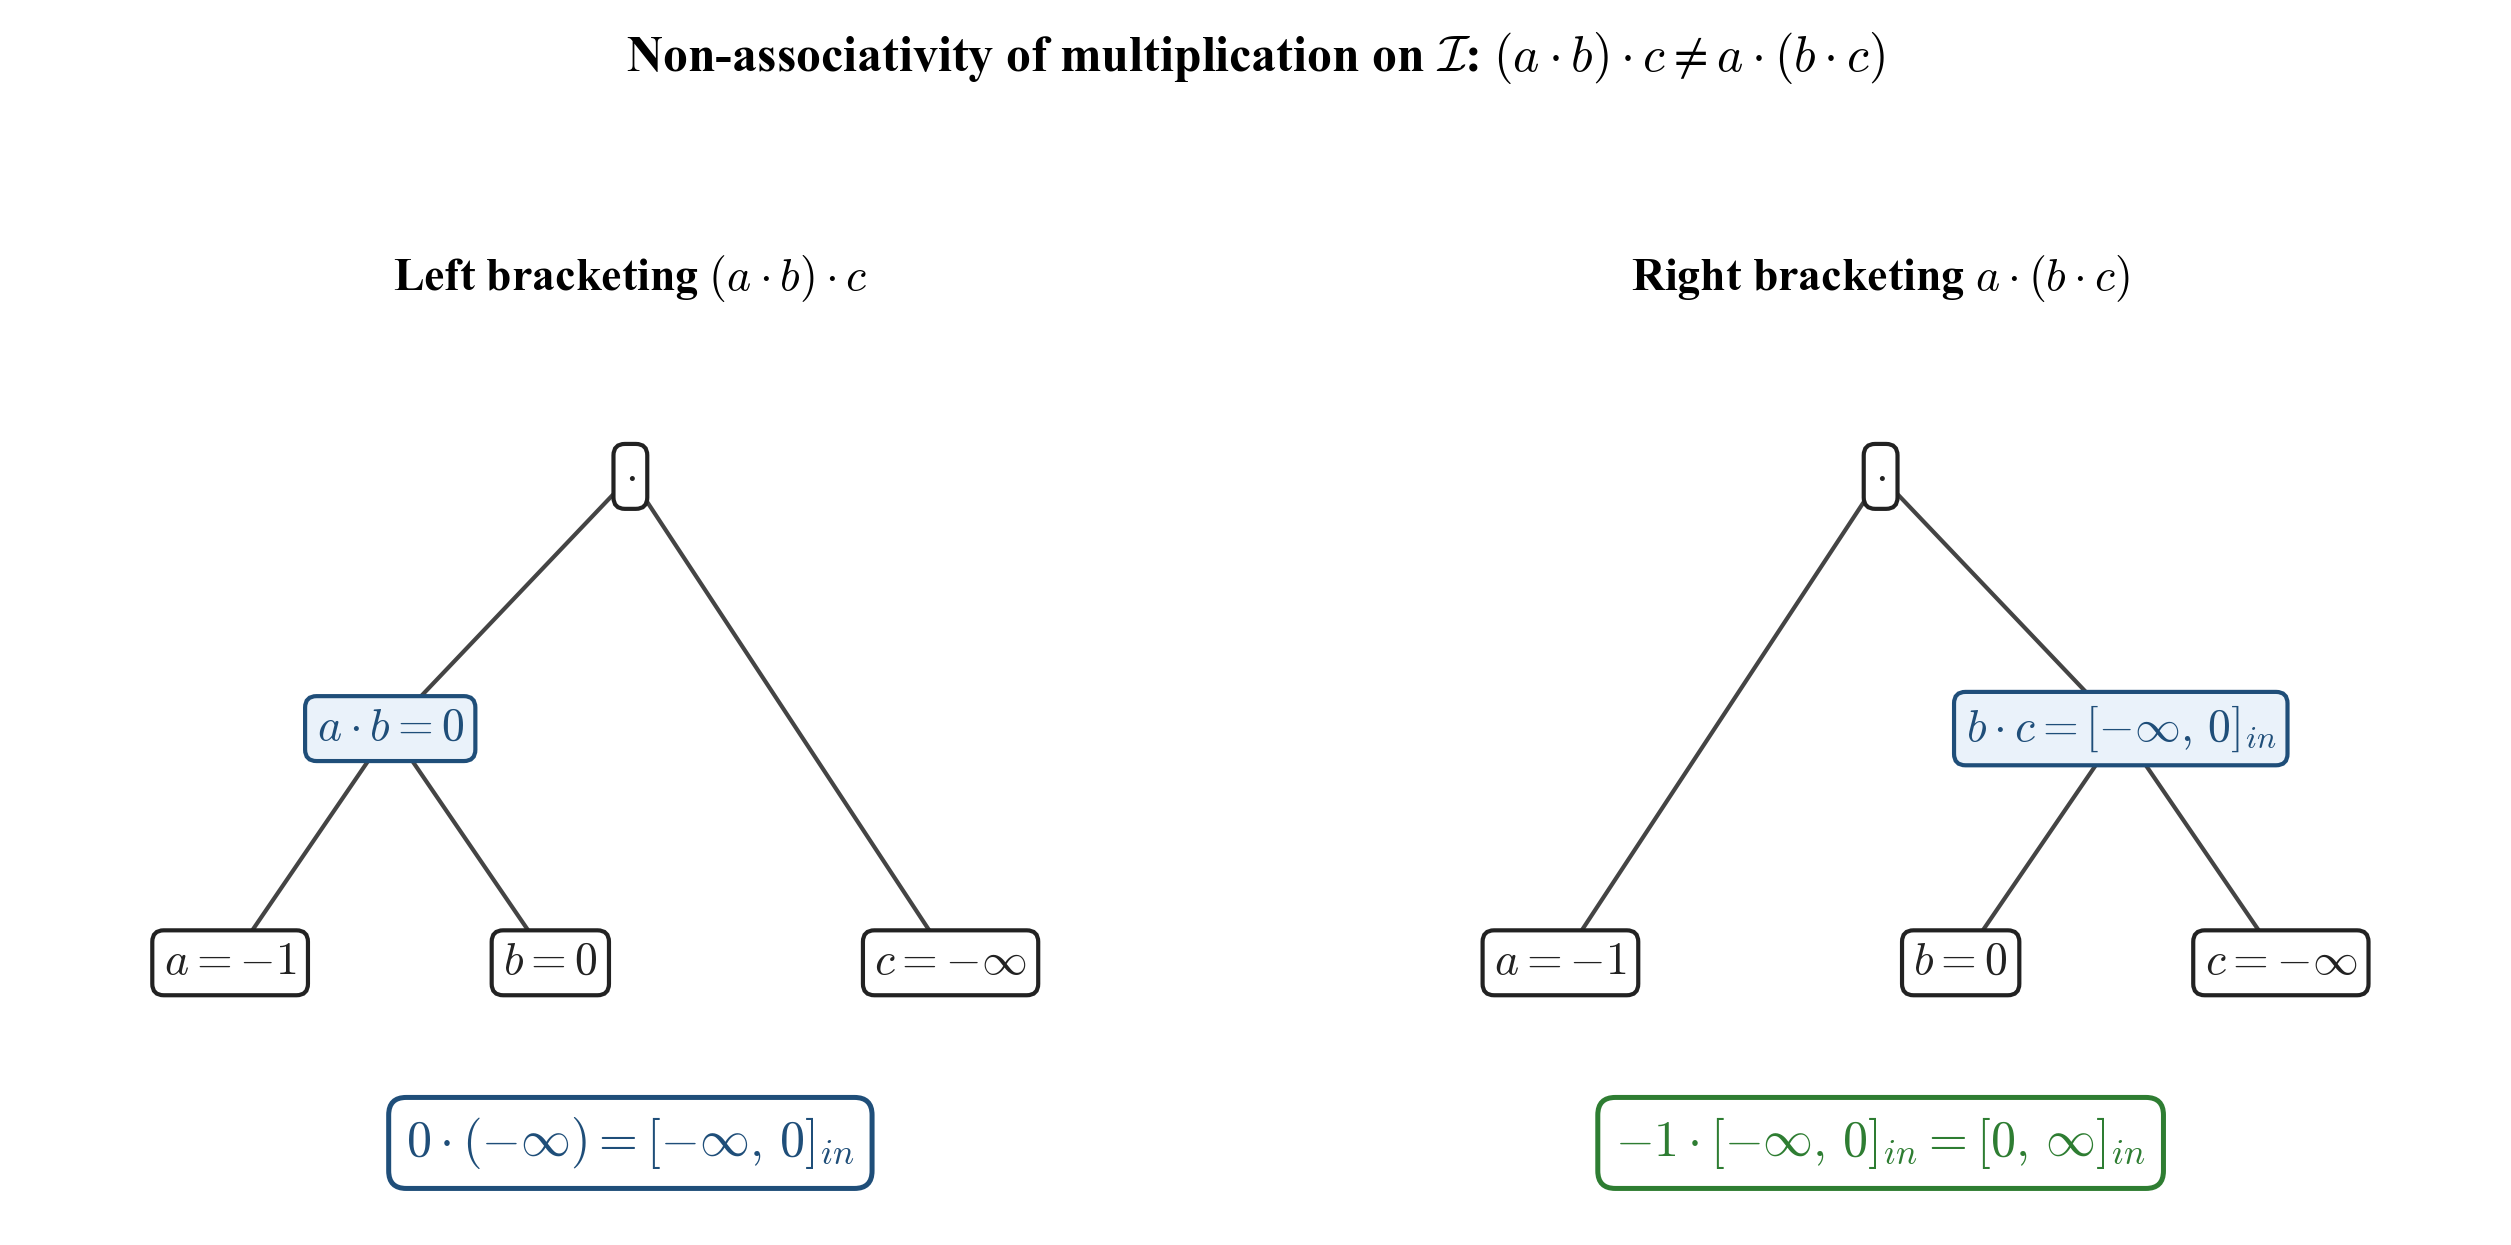
\includegraphics[width=0.85\linewidth]{fig_non_associativity.png}
  \caption{Bracketing trees for the non-associativity counterexample.
  With $a = -1$, $b = 0$, $c = -\infty$, the left bracketing
  $(a \cdot b) \cdot c$ resolves the inner product $a \cdot b = 0$
  before applying Rule~II at the outer node, yielding
  $\inI{-\infty, 0}$; the right bracketing $a \cdot (b \cdot c)$
  applies Rule~II at the inner node and then negates, yielding
  $\inI{0, \infty}$. The two results differ.}
  \label{fig:non-assoc}
\end{figure}

This counterexample is verified in the implementation by the test
\texttt{MultiplicationNotAssociative}.

The non-associativity has a precise interpretation: the bracketing of
an expression determines \emph{when} an indeterminate form is resolved
into an interval; once an interval has been formed, subsequent
multiplication propagates uncertainty rather than collapsing it. The
failure is therefore not inherited from real multiplication or from
classical (Moore) interval multiplication, both of which are
associative; it is specific to the rule by which indeterminate
symbolic forms are mapped to intervals.

\subsection{Limitations of the Structure}\label{sec:limitations}

Beyond closure and identity, the following stronger algebraic axioms
do \emph{not} hold in general:

\begin{center}
\begin{tabular}{@{}lll@{}}
\toprule
Axiom & Status & Remark \\
\midrule
Closure & \textbf{holds} & Theorem~\ref{thm:closure} \\
Multiplicative identity & \textbf{holds globally}
  & $\inI{1, 1}$ is a two-sided identity \\
Associativity & \textbf{fails}
  & Proposition~\ref{prop:non-assoc} \\
Multiplicative inverses & fails
  & intervals containing $0$ strictly admit no inverse in $\Iset$ \\
Distributivity over $+$ & fails
  & sub-distributivity holds in classical interval arithmetic
    \cite{Moore1966} \\
\bottomrule
\end{tabular}
\end{center}

The structure $(\Iset, \cdot, \inI{1,1})$ is therefore a
\textbf{unital magma}: closure and a two-sided identity hold, but
associativity fails so it is neither a semigroup nor a monoid.
Identifying maximal sub-structures on which stronger axioms recover
(e.g., associativity on point-interval subsemigroups, monoidal
behaviour on intervals bounded away from zero) is left to future
work; see Section~\ref{sec:conclusion}.

\begin{figure}[H]
  \centering
  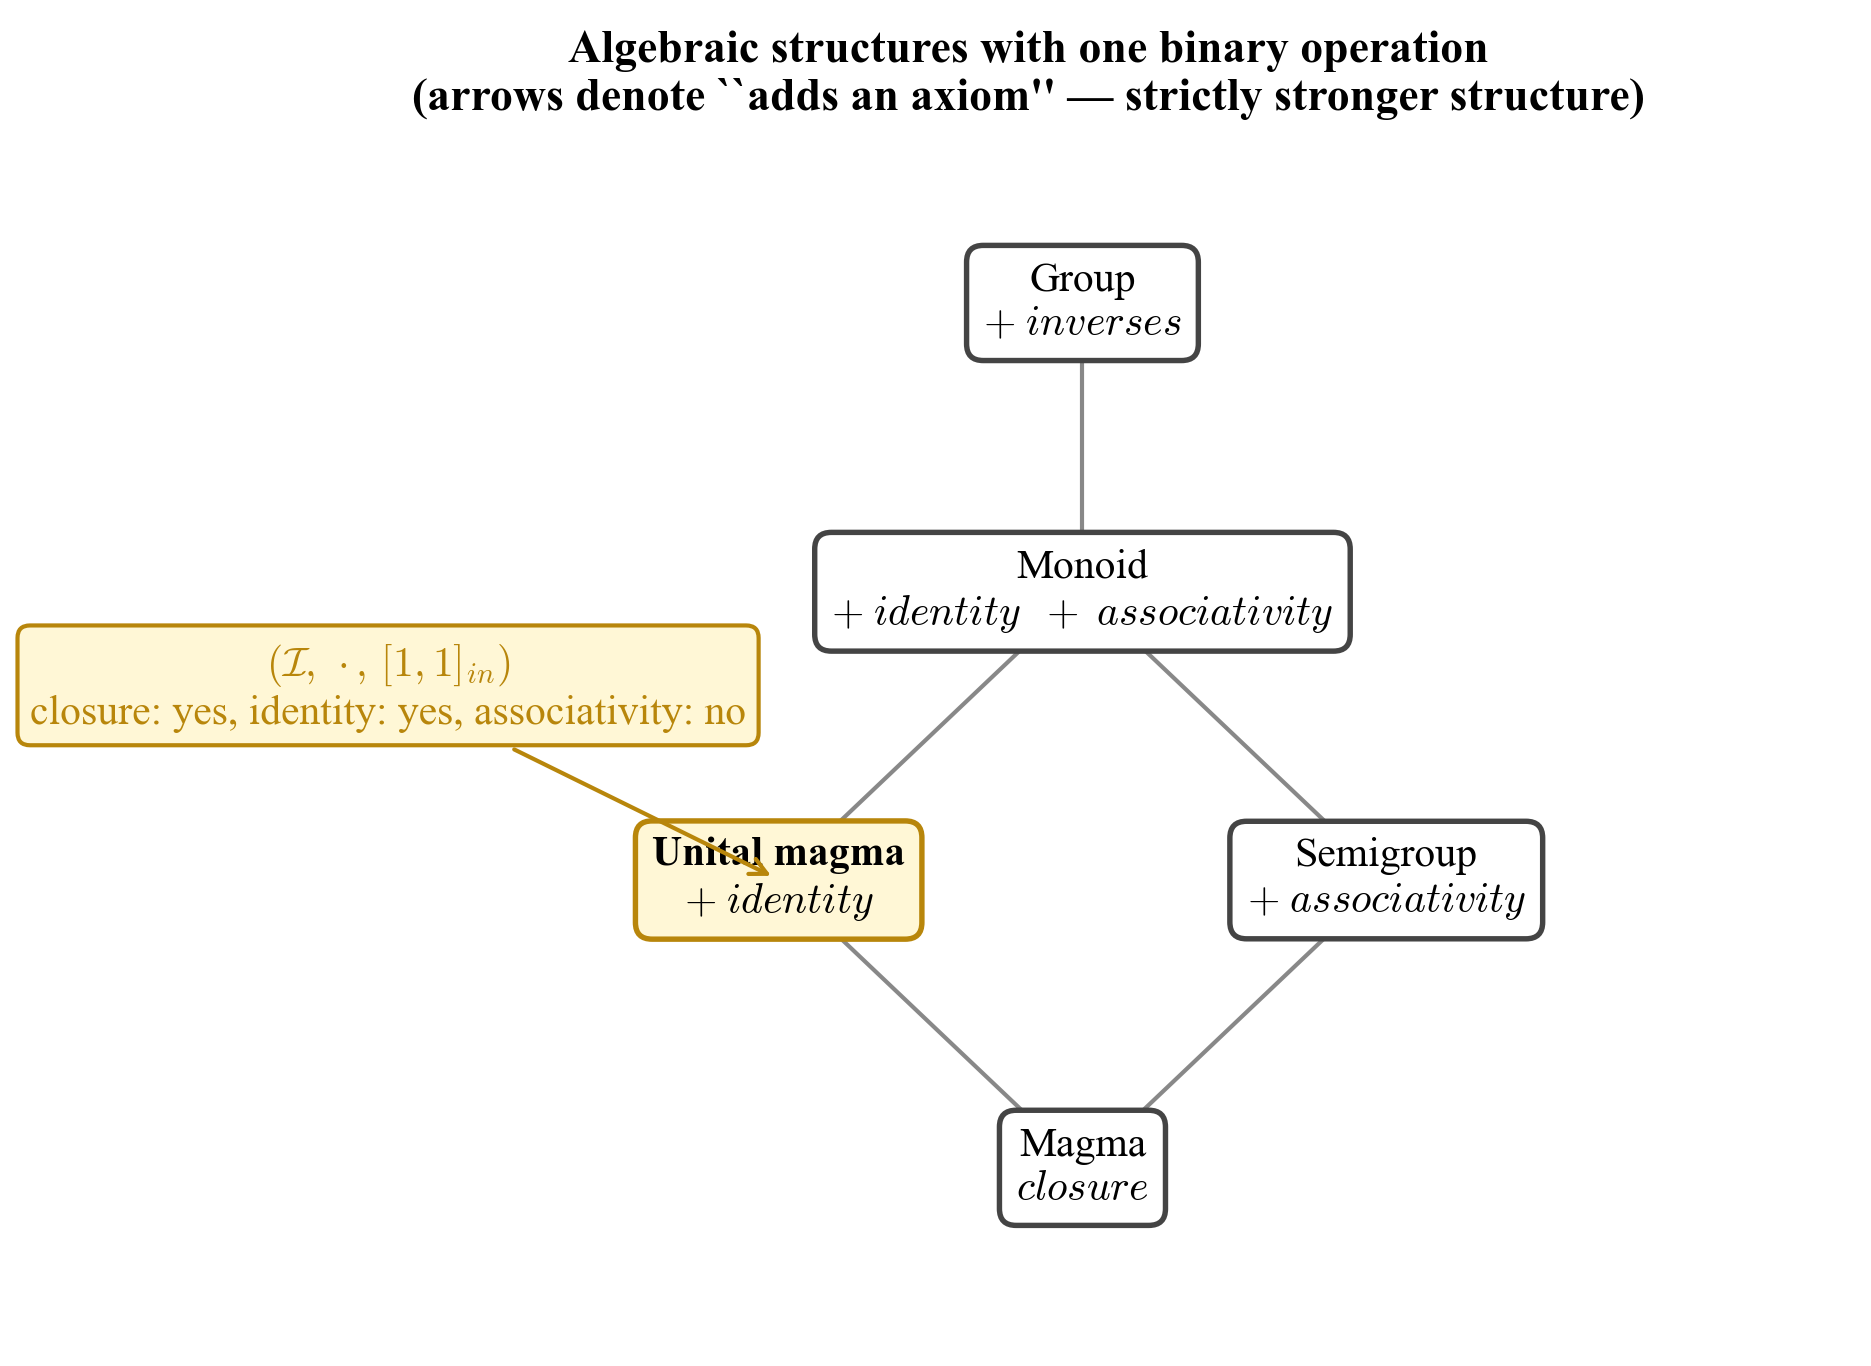
\includegraphics[width=0.7\linewidth]{fig_algebraic_hierarchy.png}
  \caption{Position of $(\Iset, \cdot, \inI{1,1})$ in the standard
  hierarchy of algebraic structures with a single binary operation.
  Each upward edge denotes the addition of an axiom (associativity,
  identity, or inverses). The structure satisfies closure and
  identity but not associativity, locating it at \textbf{unital
  magma}; it does not lift to a monoid because of the counterexample
  of Proposition~\ref{prop:non-assoc}.}
  \label{fig:hierarchy}
\end{figure}

\subsection{Significance}

Despite the limitations of Section~\ref{sec:limitations}, the
unital-magma structure is sufficient to support consistent algebraic
manipulation of indeterminate forms within bracketed expressions, as
demonstrated in Section~\ref{sec:applications}. Crucially, the
framework makes the failure of associativity \emph{visible and
meaningful} rather than hiding it behind an undefined symbol:
bracketing now corresponds to a specific algebraic choice with
computable consequences.

%====================================================================
\section{Worked Examples and Classical Forms}\label{sec:applications}

This section illustrates the framework through worked algebraic
examples and tabulates the interval-number representations of the
classical indeterminate forms together with their limit-based
justifications. No application case study from numerical analysis or
engineering is claimed here; the examples document the internal
consistency of Definitions~\ref{def:multiplication}--\ref{def:power}
with the foundation rules of Section~\ref{sec:interval-numbers}.

\subsection{Algebraic Consistency}\label{sec:algebraic-consistency}

\paragraph{Claim.}
$0 \cdot \infty = -1 \cdot (0 \cdot (-\infty))$. Equivalently,
$\Omega = -1 \cdot (-\Omega)$.

\paragraph{Derivation.}
\begin{center}
\begin{tabular}{@{}ll@{}}
\toprule
Step & Operation or Rule \\
\midrule
$-1 \cdot (0 \cdot (-\infty))$ & apply Rule II:
  $0 \cdot (-\infty) = -\Omega$ \\
$-1 \cdot \inI{-\infty, 0}$ & scalar multiplication
  (Definition~\ref{def:multiplication}) \\
$\inI{-1 \cdot 0,\ -1 \cdot (-\infty)}$ & operations in $\Rext$ \\
$\inI{0, \infty} = \Omega$ & apply Rule I \\
$0 \cdot \infty$ & $\square$ \\
\bottomrule
\end{tabular}
\end{center}

The interval-number framework therefore validates the intuitive
algebraic identity, a result not attainable with naive limit
analysis.

\subsection{Combined Operations}

\paragraph{Example~6.1.}
$\lvert \tfrac{0}{0} \rvert + \infty = \infty.$

\emph{Derivation.}
\begin{itemize}[leftmargin=2em]
  \item $\tfrac{0}{0} = \inI{-\infty, \infty}$
    (Definition~\ref{def:division});
  \item $\lvert \inI{-\infty, \infty} \rvert = \inI{0, \infty}$
    (Definition~\ref{def:abs});
  \item $\inI{0, \infty} + \infty
    = \inI{0 + \infty,\ \infty + \infty}
    = \inI{\infty, \infty} = \infty$. $\quad\square$
\end{itemize}

\paragraph{Example~6.2.}
$\tfrac{\infty}{\infty} + \infty = \infty.$

\emph{Derivation.}
\begin{itemize}[leftmargin=2em]
  \item $\tfrac{\infty}{\infty} = \inI{0, \infty}$
    (see Section~\ref{sec:classical-forms});
  \item $\inI{0, \infty} + \infty = \inI{\infty, \infty} = \infty$.
    $\quad\square$
\end{itemize}

\subsection{Classical Indeterminate Forms and Their Interval Representations}\label{sec:classical-forms}

The following table summarizes the principal indeterminate forms
together with their interval-number representations and limit-based
justifications.

\begin{center}
\renewcommand{\arraystretch}{1.35}
\begin{tabular}{@{}lll@{}}
\toprule
Form & Interval & Justification \\
\midrule
$0 \cdot \infty$ & $\inI{0, \infty}$ & Rule I \\
$0 \cdot (-\infty)$ & $\inI{-\infty, 0}$ & Rule II \\
$\dfrac{0}{0}$ & $\inI{-\infty, \infty}$
  & $\lim_{x \to 0^{+}}\tfrac{x}{x^2} = +\infty$ vs.\
    $\lim_{x \to 0^{-}}\tfrac{x}{x^2} = -\infty$ \\
$\infty - \infty$ & $\inI{-\infty, \infty}$
  & $\lim(n - n^2) = -\infty$ vs.\ $\lim(n^2 - n) = \infty$ \\
$\dfrac{\infty}{\infty}$ & $\inI{0, \infty}$
  & $\lim\tfrac{n}{n^2} = 0$ vs.\ $\lim\tfrac{n^2}{n} = \infty$ \\
$0^0$ & $\inI{0, \infty}$
  & parametric $a_n = 1/n,\ b_n = -\tfrac{\ln c}{\ln n}$
    gives $a_n^{b_n} = c$ \\
$1^\infty$ & $\inI{0, \infty}$
  & parametric $a_n = 1 + \tfrac{\ln c}{n},\ b_n = n$
    gives $a_n^{b_n} \to c$ \\
$\infty^0$ & $\inI{0, \infty}$
  & parametric $a_n = n,\ b_n = \tfrac{\ln c}{\ln n}$
    gives $a_n^{b_n} = c$ \\
\bottomrule
\end{tabular}
\end{center}

These representations are consistent with the definitions in
Section~\ref{sec:operations}: for each form, evaluating it via the
relevant Section-\ref{sec:operations} rule reproduces the listed
interval. A global soundness theorem covering all composite
expressions is not claimed; non-associativity of multiplication
(Section~\ref{sec:non-associativity}) and convex-hull approximation
in the reciprocal (Section~\ref{sec:reciprocal}) preclude such a
claim in full generality.

Using the shorthand of Section~\ref{sec:foundation-rules}, the rows
of the table can be summarized as $0 \cdot \infty = \Omega$,
$0 \cdot (-\infty) = -\Omega$, $0/0 = \widetilde{\Omega}$,
$\infty - \infty = \widetilde{\Omega}$, and
$\infty/\infty = 0^0 = 1^\infty = \infty^0 = \Omega$.

\subsection{Worked Limits Justifying Selected Intervals}

For $\dfrac{0}{0} = \inI{-\infty, \infty}$:
\[
\lim_{x \to 0^{+}}\frac{x}{x^{2}} = +\infty, \qquad
\lim_{x \to 0^{-}}\frac{x}{x^{2}} = -\infty.
\]
For any finite $c \in \mathbb{R}$, the parametric sequences
$a_n = c/n$, $b_n = 1/n$ satisfy $a_n/b_n = c$ for all $n$,
demonstrating that every value of $\mathbb{R}$ is attainable.

For $1^\infty = \inI{0, \infty}$, the endpoints are realized by
\[
\lim_{n \to \infty}\Big(1 - \tfrac{1}{\sqrt{n}}\Big)^{n^2} = 0,
\qquad
\lim_{n \to \infty}\Big(1 + \tfrac{1}{\sqrt{n}}\Big)^{n^2} = \infty,
\]
and every interior value $c \in (0, \infty)$ is attained by the
parametric witness
\[
\lim_{n \to \infty}\Big(1 + \tfrac{\ln c}{n}\Big)^{n} = e^{\ln c} = c.
\]

For $\infty^0 = \inI{0, \infty}$, the endpoints are realized by
\[
\lim_{n \to \infty} n^{-\,1/\ln\ln n} = 0, \qquad
\lim_{n \to \infty} n^{\,1/\ln\ln n} = \infty,
\]
and for every $c > 0$ the parametric witness
$a_n = n,\ b_n = (\ln c)/(\ln n)$ gives
$a_n^{b_n} = e^{\ln c} = c$ for all $n \ge 2$.

For $0^0 = \inI{0, \infty}$, for every $c > 0$ the parametric witness
$a_n = 1/n,\ b_n = -(\ln c)/(\ln n)$ satisfies
$a_n^{b_n} = n^{\ln c / \ln n} = c$ for all $n \ge 2$, while
$b_n = \pm 1/\sqrt{\ln n}$ yields the endpoints $0$ and $\infty$.

%====================================================================
\section{Conclusion and Future Work}\label{sec:conclusion}

\subsection{Summary}

This work has introduced \textbf{interval numbers} as a formal
algebraic framework for representing and manipulating indeterminate
forms. By embedding indeterminate expressions into closed intervals of
the extended real line $\Rext$, the basic arithmetic operations
(addition, subtraction, multiplication, reciprocal, division,
absolute value) are made total on $\Iset$, and exponentiation is
defined on a precisely stated admissible domain. The induced
multiplicative structure is a \textbf{unital magma}---closed, with
two-sided identity $\inI{1,1}$, but neither associative nor
monoidal---and supports consistent algebraic manipulation while
preserving the intuitive interpretation of indeterminate forms as
ranges of admissible limit values. A C++ reference implementation
accompanied by a unit test suite exercises the framework
computationally on representative cases.

\subsection{Limitations and Open Questions}

To support an honest appraisal, the principal limitations of the
framework are stated explicitly:
\begin{enumerate}[leftmargin=2em]
  \item \textbf{Multiplication is not associative.}
    Proposition~\ref{prop:non-assoc} exhibits a concrete
    counterexample. Consequently, the result of an interval-number
    expression depends on its bracketing, and the framework only
    enjoys unital-magma structure---not semigroup, monoid, or group
    structure---on $\Iset$ as a whole.

  \item \textbf{Loss of tightness for division by zero-spanning
    intervals.} When the divisor strictly contains zero, the natural
    reciprocal is a union of two intervals; to retain closure within
    $\Iset$, the framework returns $\inI{-\infty, \infty}$, which is
    sound but not tight (Section~\ref{sec:reciprocal}).

  \item \textbf{Convention behind $\tfrac{0}{0}$.}
    The reciprocal of the point interval $\inI{0,0}$ is assigned
    $\inI{-\infty, \infty}$ by the convex-hull convention of
    Definition~\ref{def:reciprocal}; the value of $\tfrac{0}{0}$ then
    follows internally from Definition~\ref{def:division}. The choice
    of $\inI{-\infty, \infty}$ for the reciprocal of $\inI{0,0}$ is a
    convention motivated by directional limits, not an internal
    derivation.

  \item \textbf{No proven distributivity.} Sub-distributivity of
    multiplication over addition holds in classical interval
    arithmetic~\cite{Moore1966}; full distributivity does not
    transfer, and a precise statement for $\Iset$ is not given here.

  \item \textbf{Choice of limit witnesses.} The interval assigned to
    each indeterminate form is justified by exhibiting limit
    sequences whose values reach (or approach) the endpoints. A proof
    that the chosen interval is \emph{optimal}---i.e., that no
    admissible value lies strictly outside it---is informal and rests
    on standard real-analytic intuition rather than a fully formal
    argument.

  \item \textbf{Floating-point realization.} Any numerical
    realization (such as the reference implementation) inherits the
    rounding behaviour of its arithmetic substrate. The mathematical
    claims are stated in $\Rext$; floating-point realizations are
    approximate.
\end{enumerate}

These limitations delineate the scope of the present contribution and
motivate the directions outlined in Section~\ref{sec:future}.

\subsection{Future Directions}\label{sec:future}

The interval-number framework opens several avenues for further
investigation:
\begin{enumerate}[leftmargin=2em]
  \item \textbf{Richer algebraic structure.} Investigate whether
    interval numbers exhibit additional structure (associativity,
    distributivity, identities, inverses) under suitable
    restrictions---for example, on intervals not containing zero, or
    on the set of point intervals.

  \item \textbf{Measure-theoretic integration.} Reconcile
    interval-number operations with measure-theoretic conventions for
    handling indeterminate forms~\cite{Folland1999}, where
    context-specific conventions such as $0 \cdot \infty = 0$ are
    common.

  \item \textbf{Applications.} Explore applications in:
    \begin{itemize}[leftmargin=2em]
      \item numerical analysis (controlled treatment of overflow and
        underflow),
      \item complex analysis (extension to complex-valued interval
        numbers),
      \item probability and statistics (representing imprecise
        probabilities).
    \end{itemize}

  \item \textbf{Extended operations.} Define and characterize
    additional operations on interval numbers, including:
    \begin{itemize}[leftmargin=2em]
      \item logarithm and exponential,
      \item trigonometric and hyperbolic functions,
      \item transcendental functions and their inverses.
    \end{itemize}

  \item \textbf{Categorical perspective.} Examine interval numbers
    from a categorical or topos-theoretic viewpoint to uncover deeper
    structural properties and connections with related frameworks
    (fuzzy sets, rough sets, interval-valued probabilities).

  \item \textbf{Formal verification.} Mechanize the theory in a proof
    assistant (Coq, Lean, Isabelle) to obtain machine-checked
    guarantees of soundness for all operations and identities.

  \item \textbf{Estimation of additional indeterminate intervals.}
    Other indeterminate forms---possibly arising in specific
    application domains---could be assigned interval representations
    through the same limit-based justification methodology employed
    here.

  \item \textbf{Closure of exponentiation.} Exponentiation is defined
    here only on the admissible domain stated in
    Section~\ref{sec:exponentiation}; outside that domain it remains
    partial. Extending the operation to a total map on $\Iset$
    ---either by enlarging the admissible domain through additional
    value-map cases or by adopting a closure convention analogous to
    the convex-hull convention used for the reciprocal of a
    zero-spanning interval---is left for future work.
\end{enumerate}

\subsection{Closing Remark}

While the immediate significance of the framework remains
theoretical, it offers a mathematically principled approach to a
long-standing problem in real analysis. The unification of interval
arithmetic and extended-real semantics provides a foundation upon
which further algebraic, computational, and applied investigations
can be built.

%====================================================================
\begin{thebibliography}{99}
\addcontentsline{toc}{section}{References}

\bibitem{Apostol1974}
T.~M. Apostol.
\newblock \emph{Mathematical Analysis}, 2nd ed.
\newblock Addison-Wesley, Reading, MA, 1974.

\bibitem{Folland1999}
G.~B. Folland.
\newblock \emph{Real Analysis: Modern Techniques and Their
Applications}, 2nd ed.
\newblock Wiley-Interscience, New York, 1999.

\bibitem{RockafellarWets1998}
R.~T. Rockafellar and R.~J.-B. Wets.
\newblock \emph{Variational Analysis}.
\newblock Grundlehren der mathematischen Wissenschaften, vol.~317,
Springer, Berlin, 1998.

\bibitem{Bourbaki1989}
N.~Bourbaki.
\newblock \emph{Algebra~I: Chapters 1--3}.
\newblock Elements of Mathematics, Springer-Verlag, Berlin, 1989.

\bibitem{MacLaneBirkhoff1999}
S.~Mac~Lane and G.~Birkhoff.
\newblock \emph{Algebra}, 3rd ed.
\newblock AMS Chelsea Publishing, 1999.

\bibitem{Moore1966}
R.~E. Moore.
\newblock \emph{Interval Analysis}.
\newblock Prentice-Hall, Englewood Cliffs, NJ, 1966.

\bibitem{Moore2009}
R.~E. Moore, R.~B. Kearfott, and M.~J. Cloud.
\newblock \emph{Introduction to Interval Analysis}.
\newblock SIAM, Philadelphia, 2009.
\newblock \href{https://doi.org/10.1137/1.9780898717716}{doi:10.1137/1.9780898717716}.

\bibitem{Neumaier1990}
A.~Neumaier.
\newblock \emph{Interval Methods for Systems of Equations}.
\newblock Encyclopedia of Mathematics and its Applications, vol.~37,
Cambridge University Press, 1990.

\bibitem{IEEE1788}
IEEE Standard for Interval Arithmetic, IEEE Std~1788-2015.
\newblock IEEE, New York, 2015.
\newblock \href{https://doi.org/10.1109/IEEESTD.2015.7140721}{doi:10.1109/IEEESTD.2015.7140721}.

\bibitem{Kaucher1980}
E.~Kaucher.
\newblock Interval analysis in the extended interval space~$\mathbb{IR}$.
\newblock \emph{Computing Supplementum} 2, 33--49, Springer-Verlag,
Vienna, 1980.
\newblock \href{https://doi.org/10.1007/978-3-7091-8577-3_3}{doi:10.1007/978-3-7091-8577-3\_3}.

\bibitem{HansenWalster2004}
E.~Hansen and G.~W. Walster.
\newblock \emph{Global Optimization Using Interval Analysis}, 2nd ed.,
revised and expanded.
\newblock Marcel Dekker / CRC Press, New York, 2004.

\bibitem{Carlstroem2004}
J.~Carlstr\"om.
\newblock Wheels---On division by zero.
\newblock \emph{Mathematical Structures in Computer Science} 14(1),
143--184, 2004.
\newblock \href{https://doi.org/10.1017/S0960129503004110}{doi:10.1017/S0960129503004110}.

\bibitem{BergstraTucker2007}
J.~A. Bergstra and J.~V. Tucker.
\newblock The rational numbers as an abstract data type.
\newblock \emph{Journal of the ACM} 54(2), Article~7, 2007.
\newblock \href{https://doi.org/10.1145/1219092.1219095}{doi:10.1145/1219092.1219095}.

\end{thebibliography}

\end{document}
